\documentclass[5p,times,twocolumn]{elsarticle}

%\usepackage{lineno}
\usepackage{graphicx}
\usepackage{amsmath,amssymb}
\usepackage{booktabs}
\usepackage{multirow}
\usepackage{tabularx}
\usepackage{array}
\usepackage{algorithm}
\usepackage{algorithmic}
\usepackage{url}
\usepackage{hyperref}

\journal{Energy and Buildings}

\bibliographystyle{elsarticle-num-names}

\begin{document}

\begin{frontmatter}

\title{From Static Shading to Time-Domain Control: A Unified Solar-Thermal-Adaptive Framework for Climate-Adaptive Passive Building Design}

\author[inst1]{Author Name\corref{corresponding}}
\cortext[corresponding]{Corresponding author}
\affiliation[inst1]{organization={Department of Architecture, University Name},
                   city={City},
                   country={Country}}

\begin{abstract}
The building sector remains a major target for decarbonization and climate adaptation, yet passive solar design is still frequently implemented through static shading rules, steady-state envelope metrics, or reactive operational logic. Such fragmented treatments are increasingly insufficient for buildings exposed to anisotropic sky conditions, transient heat storage and release, and highly variable internal disturbances. This paper proposes a Unified Solar-Thermal-Adaptive (USTA) framework that reformulates passive solar design as a time-domain, climate-adaptive decision problem. The framework couples anisotropic solar admission modeling, reduced-order transient thermal dynamics, multi-objective passive design optimization, and predictive facade control within a single physics-informed pipeline. In contrast to conventional noon-based or purely geometric approaches, USTA explicitly captures diffuse sky structure, thermal lag, and anticipatory control requirements under variable occupancy. The resulting formulation supports warm-climate solar rejection, cold-climate solar storage and survivability analysis, adaptive operation for stochastic-use buildings, and transferable design synthesis across latitudes and facade orientations. By combining physical interpretability with computational efficiency, the proposed framework provides a unified basis for passive-first retrofit and new-building design under heterogeneous climatic and operational conditions.
\end{abstract}

\begin{keyword}
Passive Solar Design \sep Anisotropic Sky Model \sep 3R2C Thermal Network \sep Model Predictive Control \sep Multi-Objective Optimization \sep NSGA-II \sep Climate-Adaptive Buildings \sep Thermal Inertia \sep Kinetic Facade \sep Thermal Resilience
\end{keyword}

\end{frontmatter}

%\linenumbers

\section{Introduction}
\label{sec:introduction}

Buildings remain one of the largest contributors to global energy demand and carbon emissions. According to UNEP, the buildings and construction sector accounted for 34\% of global energy demand and 37\% of energy- and process-related CO$_2$ emissions in 2022, making building decarbonization and climate adaptation a first-order research priority rather than a secondary design concern \cite{unep2024}. In this context, passive solar design has regained strategic importance because it can reduce operational dependence on mechanical systems while improving climate responsiveness at the envelope level.

Existing passive design work largely treats solar shading, building thermal performance, and operational control as separate concerns. Studies on shading devices optimize fixed geometries against cooling or daylight criteria \cite{kirimtat2016,valladares2014,nazari2023}; thermal modeling work characterizes envelope properties in quasi-steady state \cite{verbeke2018,yang2024,lauster2014}; and building control research applies predictive methods to HVAC systems without tightly coupling them to upstream passive design decisions \cite{drgona2020,zhan2021}. Each of these lines has produced valuable insights, but together they reflect a fragmented view of what is fundamentally an integrated problem. We argue that climate-adaptive passive design should instead be treated as a unified time-domain problem --- one in which solar admission decisions, thermal storage behavior, and operational adaptation are formulated within a single physical model and optimized jointly across design time and run time.

Pursuing this integrated vision, however, surfaces two non-trivial challenges. The first is radiative fidelity: when the goal is to evaluate design decisions against the full distribution of hourly sky states rather than a representative sun angle, the isotropic diffuse assumptions that suffice for steady-state reasoning become inadequate. Diffuse radiation, circumsolar brightening, and horizon effects can substantially alter the irradiance on tilted facades at the hours that most affect peak loads \cite{perez1990}, so the solar input model must be both time-resolved and anisotropically accurate. The second challenge is bridging time scales: passive design decisions are set before occupancy is known and must remain durable across seasons, whereas operational control decisions respond to real-time disturbances over horizons of hours \cite{goncalves2024,hong2023,ismail2023}. Coupling these two decision layers within a single computationally tractable formulation --- without losing the physical consistency that makes the coupled model meaningful --- is not straightforward.

To address the first challenge, we introduce a time-resolved solar admission layer grounded in the Perez anisotropic sky model, coupled to a 3R2C reduced-order transient thermal network; this pairing captures storage, delay, and survivability effects while remaining computationally efficient and physically interpretable. To address the second challenge, we formulate the design-control pipeline as a bi-level problem: an offline layer driven by multi-objective optimization selects durable design parameters from a Pareto-efficient solution set, and an online layer driven by model predictive control adapts controllable facade and HVAC decisions in anticipation of near-term thermal loads --- both layers sharing the same underlying physical model. The resulting Unified Solar-Thermal-Adaptive (USTA) framework is evaluated across four case studies spanning warm-climate shading, cold-climate passive heating, variable-occupancy adaptive control, and cross-latitude design generalization. USTA achieves a 35.7\% reduction in annual heating demand, a 94.1\% comfort-hour rate under dynamic occupancy, and a 45\% improvement in passive survivability during simulated grid outage.

The main contributions of this paper are threefold. First, we formulate climate-adaptive passive building design as a unified bi-level optimization-control problem, coupling design variables and control variables through a shared physical model and making explicit the structural relationship between design-time decisions and run-time performance. Second, we integrate a Perez anisotropic sky model for time-resolved solar admission with a 3R2C transient thermal network, providing a model chain that is both physically interpretable and efficient enough to serve as the shared representation for multi-objective offline optimization and online predictive control. Third, we provide systematic cross-scenario validation with ablation experiments that isolate the contribution of each framework component across cooling-dominated, heating-dominated, occupancy-variable, and multi-latitude conditions, offering replicable evidence for the performance value of solar-thermal-control integration in passive building design.

The rest of this paper is organized as follows. Section \ref{sec:related} reviews prior work on shading and solar-admission modeling, reduced-order thermal modeling, and predictive control and dynamic facades. Section \ref{sec:formulation} formulates the proposed USTA framework mathematically. Section \ref{sec:method} presents the optimization and control pipeline. Section \ref{sec:setup} describes the experimental setup and baselines. Section \ref{sec:results} presents results across four case studies. Section \ref{sec:ablation} provides ablation and sensitivity analysis. Section \ref{sec:discussion} discusses implications and limitations. Section \ref{sec:conclusion} concludes.

\section{Related Work}
\label{sec:related}

\subsection{Static Shading Design and Solar-Admission Modelling}

Solar shading has long been recognized as one of the most important passive means for reducing cooling load, mitigating glare, and improving facade energy performance. Review studies have documented a wide range of shading devices, simulation methods, and performance criteria across climates and building types \cite{kirimtat2016}. Representative application studies have shown that fixed overhangs, fins, and spectrally selective configurations can reduce solar gains while balancing visual comfort and daylight access \cite{valladares2014,nazari2023}. This literature has been highly valuable for identifying facade-level trade-offs, but its dominant modeling pattern is still largely configuration-oriented: optimize a fixed device, compare a set of facade alternatives, or assess one climate-specific shading package. Such formulations are useful for local design decisions, yet they do not fully resolve the deeper problem of time-varying solar admission under anisotropic sky conditions. The Perez model is foundational here because it explicitly models diffuse irradiance on tilted planes under all-weather conditions, including circumsolar and horizon effects that simplified geometric reasoning tends to suppress \cite{perez1990}. Our work builds on this insight but moves further by embedding anisotropic solar admission inside a larger transient decision framework.

\subsection{Thermal Inertia, Transient Response, and Reduced-Order Models}

A parallel literature has established that building performance is strongly shaped by thermal inertia and by the timing, not merely the magnitude, of heat transfer. Review work by Verbeke and Audenaert shows that thermal mass can time-shift and flatten heat-flow fluctuations, although its performance varies substantially with climate, insulation, and building use \cite{verbeke2018}. More recent RC-model reviews emphasize that low-order resistance-capacitance models offer a practical compromise between physical meaning and computational tractability, making them especially suitable for fast simulation, early design, and control-oriented prediction \cite{yang2024}. Earlier studies on low-order thermal networks likewise argue that dynamic building behavior can be captured by reduced numbers of resistances and capacitances at low computational cost, in contrast to higher-order methods whose parameterization and runtime burdens are often prohibitive for design iteration \cite{lauster2014}. These works provide the methodological foundation for using 3R2C-style state representations in passive design research. At the same time, much of the thermal-inertia literature stops at dynamic analysis or performance explanation. Our framework takes the next step by directly coupling thermal storage and release to time-resolved solar admission and adaptive facade decisions.

\subsection{Predictive Control, Dynamic Facades, and Resilience-Oriented Operation}

The building-control literature has demonstrated that MPC is one of the most systematic ways to coordinate comfort, energy use, forecasts, and operational constraints \cite{drgona2020}. However, review studies also make clear that the practical deployment of MPC still depends critically on obtaining suitable control-oriented models and understanding the relationship between model quality, data requirements, and final control performance \cite{zhan2021}. Meanwhile, research on dynamic facades has expanded rapidly. Recent systematic reviews describe dynamic facades as a promising response to the mismatch between static envelopes and dynamic external stimuli, with reported benefits in thermal comfort, energy efficiency, and daylight performance \cite{goncalves2024}. Yet this line of work often concentrates on facade technologies or actuation logic, while leaving the building's internal thermal storage and survivability behavior only loosely connected to the facade decision process. At the same time, resilience-oriented studies increasingly evaluate passive survivability, habitable hours, and outage performance under extreme events \cite{hong2023,ismail2023}. These studies highlight an important shift in performance criteria, but they also reveal that resilience metrics are still often used as evaluation endpoints rather than as native objectives in a unified passive design-and-operation framework. Our work responds to this gap by treating adaptive control and resilience as integral parts of passive solar design.

\subsection{Positioning of This Work}

In summary, existing studies provide strong but still separated answers to three different questions: how to reduce solar gains with facade devices \cite{kirimtat2016,perez1990,valladares2014,nazari2023}, how to represent transient thermal storage and release efficiently \cite{verbeke2018,yang2024,lauster2014}, and how to optimize building operation under forecasts and constraints \cite{drgona2020,zhan2021,goncalves2024}. What remains insufficiently addressed is the joint formulation of these questions as one coherent passive-first decision problem. The proposed USTA framework is positioned precisely at this intersection. Rather than optimizing shading alone, simulating thermal mass alone, or controlling a facade alone, USTA unifies anisotropic solar modeling, reduced-order transient thermal dynamics, multi-objective passive design, and predictive adaptive operation within one transferable framework. This is the main distinction between our work and the existing literature.

\section{Problem Formulation}
\label{sec:formulation}

We reformulate passive solar building design as a time-domain sequential decision problem with clearly defined inputs, states, controls, constraints, and multi-objective cost functions. This formulation enables the USTA framework to be treated as a computational method rather than an engineering rule-of-thumb collection.

\subsection{Sets, Time Discretization, and Notation}

Let $\mathcal{T} = \{0, 1, \ldots, N\}$ denote the discrete time index set with uniform time step $\Delta t$ (e.g., 15 min), giving a total simulation horizon of one typical meteorological year ($N = 365 \times 24 \times 4 = 35,040$ steps). Let $\mathcal{F} = \{N, E, S, W\}$ be the set of facade orientations, each characterized by tilt angle $\beta_f$ and azimuth $\gamma_f$. For a single thermal zone with the 3R2C approximation, the state dimension is $n_x = 2$. Key notation is summarized in Table \ref{tab:notation}.

\begin{table}[!t]
\centering
\footnotesize
\caption{Mathematical notation used throughout the paper.}
\label{tab:notation}
\begin{tabularx}{\columnwidth}{@{} l >{\raggedright\arraybackslash}X l @{}}
\toprule
\textbf{Symbol} & \textbf{Description} & \textbf{Unit} \\
\midrule
$\mathcal{T}$ & Discrete time index set $\{0,1,\ldots,N\}$ & -- \\
$\Delta t$ & Time step & min \\
$\mathcal{F}$ & Set of facade orientations & -- \\
$n_x$ & State dimension (= 2 for 3R2C) & -- \\
$w_t$ & Weather input vector at time $t$ & various \\
$x_t = [T_{in}, T_m]$ & State: indoor air temp., thermal mass temp. & $^\circ$C \\
$z$ & Design variable vector (offline) & various \\
$u_t = [\theta_{lou}, s_{night}, P_{hvac}]$ & Online control vector at time $t$ & deg, --, W \\
$J = [J_e, J_c, J_g, J_s, J_a]$ & Multi-objective cost vector & various \\
$H$ & MPC prediction horizon & steps \\
\bottomrule
\end{tabularx}
\end{table}

\subsection{Input, State, and Control Variables}

At each time step $t$, the exogenous weather input is defined as:
\begin{equation}
\label{eq:weather}
w_t = [T_{out,t}, DNI_t, DHI_t, GHI_t, v_{wind,t}, \rho_{sky,t}]^T
\end{equation}
where DNI, DHI, and GHI denote direct normal, diffuse horizontal, and global horizontal irradiance respectively. These are obtained from TMY3 data files \cite{wilcox2008}. In addition, a predicted occupancy disturbance sequence $\hat{o}_{t:t+H-1}$ is provided to the MPC at each step.

The system state is defined as the 3R2C state vector:
\begin{equation}
\label{eq:state}
x_t = [T_{in,t}, T_{m,t}]^T
\end{equation}
where $T_{in,t}$ is the indoor air temperature and $T_{m,t}$ is the equivalent thermal mass temperature.

Decision variables are split into two layers:

\textbf{Design layer (offline, once per project):} $z \in \mathcal{Z}$, comprising fixed overhang depth ratio $r_{oh} = d_{oh}/h_{win}$, vertical fin depth, glazing SHGC and VLT, thermal mass scaling factor $k_C$, and maximum night insulation resistance multiplier $k_R^{max}$.

\textbf{Operation layer (online, time-varying):} $u_t = [\theta_{lou,t}, s_{night,t}, P_{hvac,t}]^T$, where $\theta_{lou,t}$ is the louver angle (continuous, $[\theta_{min}, \theta_{max}]$), $s_{night,t} \in \{0,1\}$ is the night insulation state, and $P_{hvac,t}$ is the HVAC power (set to zero in passive-survivability scenarios).

\subsection{Constraints}
\label{sec:constraints}

The following constraints are imposed:

\begin{enumerate}
\item \textbf{Thermal comfort (soft, occupied hours $\mathcal{T}_{occ}$):} $T_{low,t} \leq T_{in,t} \leq T_{high,t}$ for all $t \in \mathcal{T}_{occ}$. Soft violations are penalized via slack variables $\xi_t \geq 0$.

\item \textbf{Actuator bounds and rate limits:} $\theta_{min} \leq \theta_{lou,t} \leq \theta_{max}$; $|\theta_{lou,t} - \theta_{lou,t-1}| \leq \Delta\theta_{max}$.

\item \textbf{Night insulation:} $s_{night,t} \in \{0,1\}$ (MIQP) or $s_{night,t} \in [0,1]$ (convex relaxation).

\item \textbf{Glare:} $DGI_t \leq 22$ during occupied hours (Daylight Glare Index threshold \cite{wienold2006}).

\item \textbf{Passive survivability (outage scenario $\mathcal{T}_{out} \subset \mathcal{T}$):} $P_{hvac,t} = 0$ and $T_{in,t} \geq T_{safe}$ for all $t \in \mathcal{T}_{out}$.
\end{enumerate}

\subsection{Multi-Objective Cost Function}

We define a five-dimensional objective vector $J = [J_e, J_c, J_g, J_s, J_a]^T$:

\begin{align}
\label{eq:energy}
J_e &= \sum_{t \in \mathcal{T}} P_{hvac,t} \cdot \Delta t \\
\label{eq:comfort}
J_c &= \sum_{t \in \mathcal{T}_{occ}} \left( \max(0, T_{in,t} - T_{high,t})^2 + \max(0, T_{low,t} - T_{in,t})^2 \right) \cdot \Delta t \\
\label{eq:glare}
J_g &= \sum_{t \in \mathcal{T}_{occ}} \max(0, DGI_t - 22) \cdot \Delta t \\
\label{eq:survivability}
J_s &= \sum_{t \in \mathcal{T}_{out}} \max(0, T_{safe} - T_{in,t}) \cdot \Delta t \\
\label{eq:actuation}
J_a &= \sum_{t \in \mathcal{T}} \|u_t - u_{t-1}\|_2^2
\end{align}

\subsection{Bi-Level Optimization Formulation}

USTA is formulated as a bi-level optimization problem. The outer (design) layer seeks the Pareto-optimal design set:
\begin{equation}
\label{eq:pareto}
\mathcal{P}^* = \{ z \in \mathcal{Z} \mid \nexists z' \text{ s.t. } J(z', \pi^*_{z'}) \text{ dominates } J(z, \pi^*_z) \}
\end{equation}
where $\pi^*_z$ denotes the optimal operational policy given design $z$, produced by the inner (MPC) layer.

The inner layer solves a receding-horizon optimal control problem at each step $t$:
\begin{equation}
\label{eq:mpc}
\begin{aligned}
\min_{u_{t:t+H-1}} \quad & \sum_{k=0}^{H-1} \left[ \|x_{t+k|t} - x_{ref,t+k}\|_Q^2 + \|\Delta u_{t+k|t}\|_R^2 \right. \\
& \left. \quad + \lambda_g \cdot \phi(DGI_{t+k|t}) + \lambda_e \cdot \psi(P_{hvac,t+k|t}) \right] \\
\text{s.t.} \quad & x_{t+k+1|t} = f_d(x_{t+k|t}, u_{t+k|t}, \hat{d}_{t+k|t}; z)
\end{aligned}
\end{equation}

\section{The USTA Framework: Proposed Method}
\label{sec:method}

The USTA framework processes weather inputs through three sequential computational layers---radiation transposition, thermal state dynamics, and hierarchical optimization/control---as illustrated in Figure \ref{fig:framework}. Each layer is described below.

\begin{figure*}[!t]
\centering
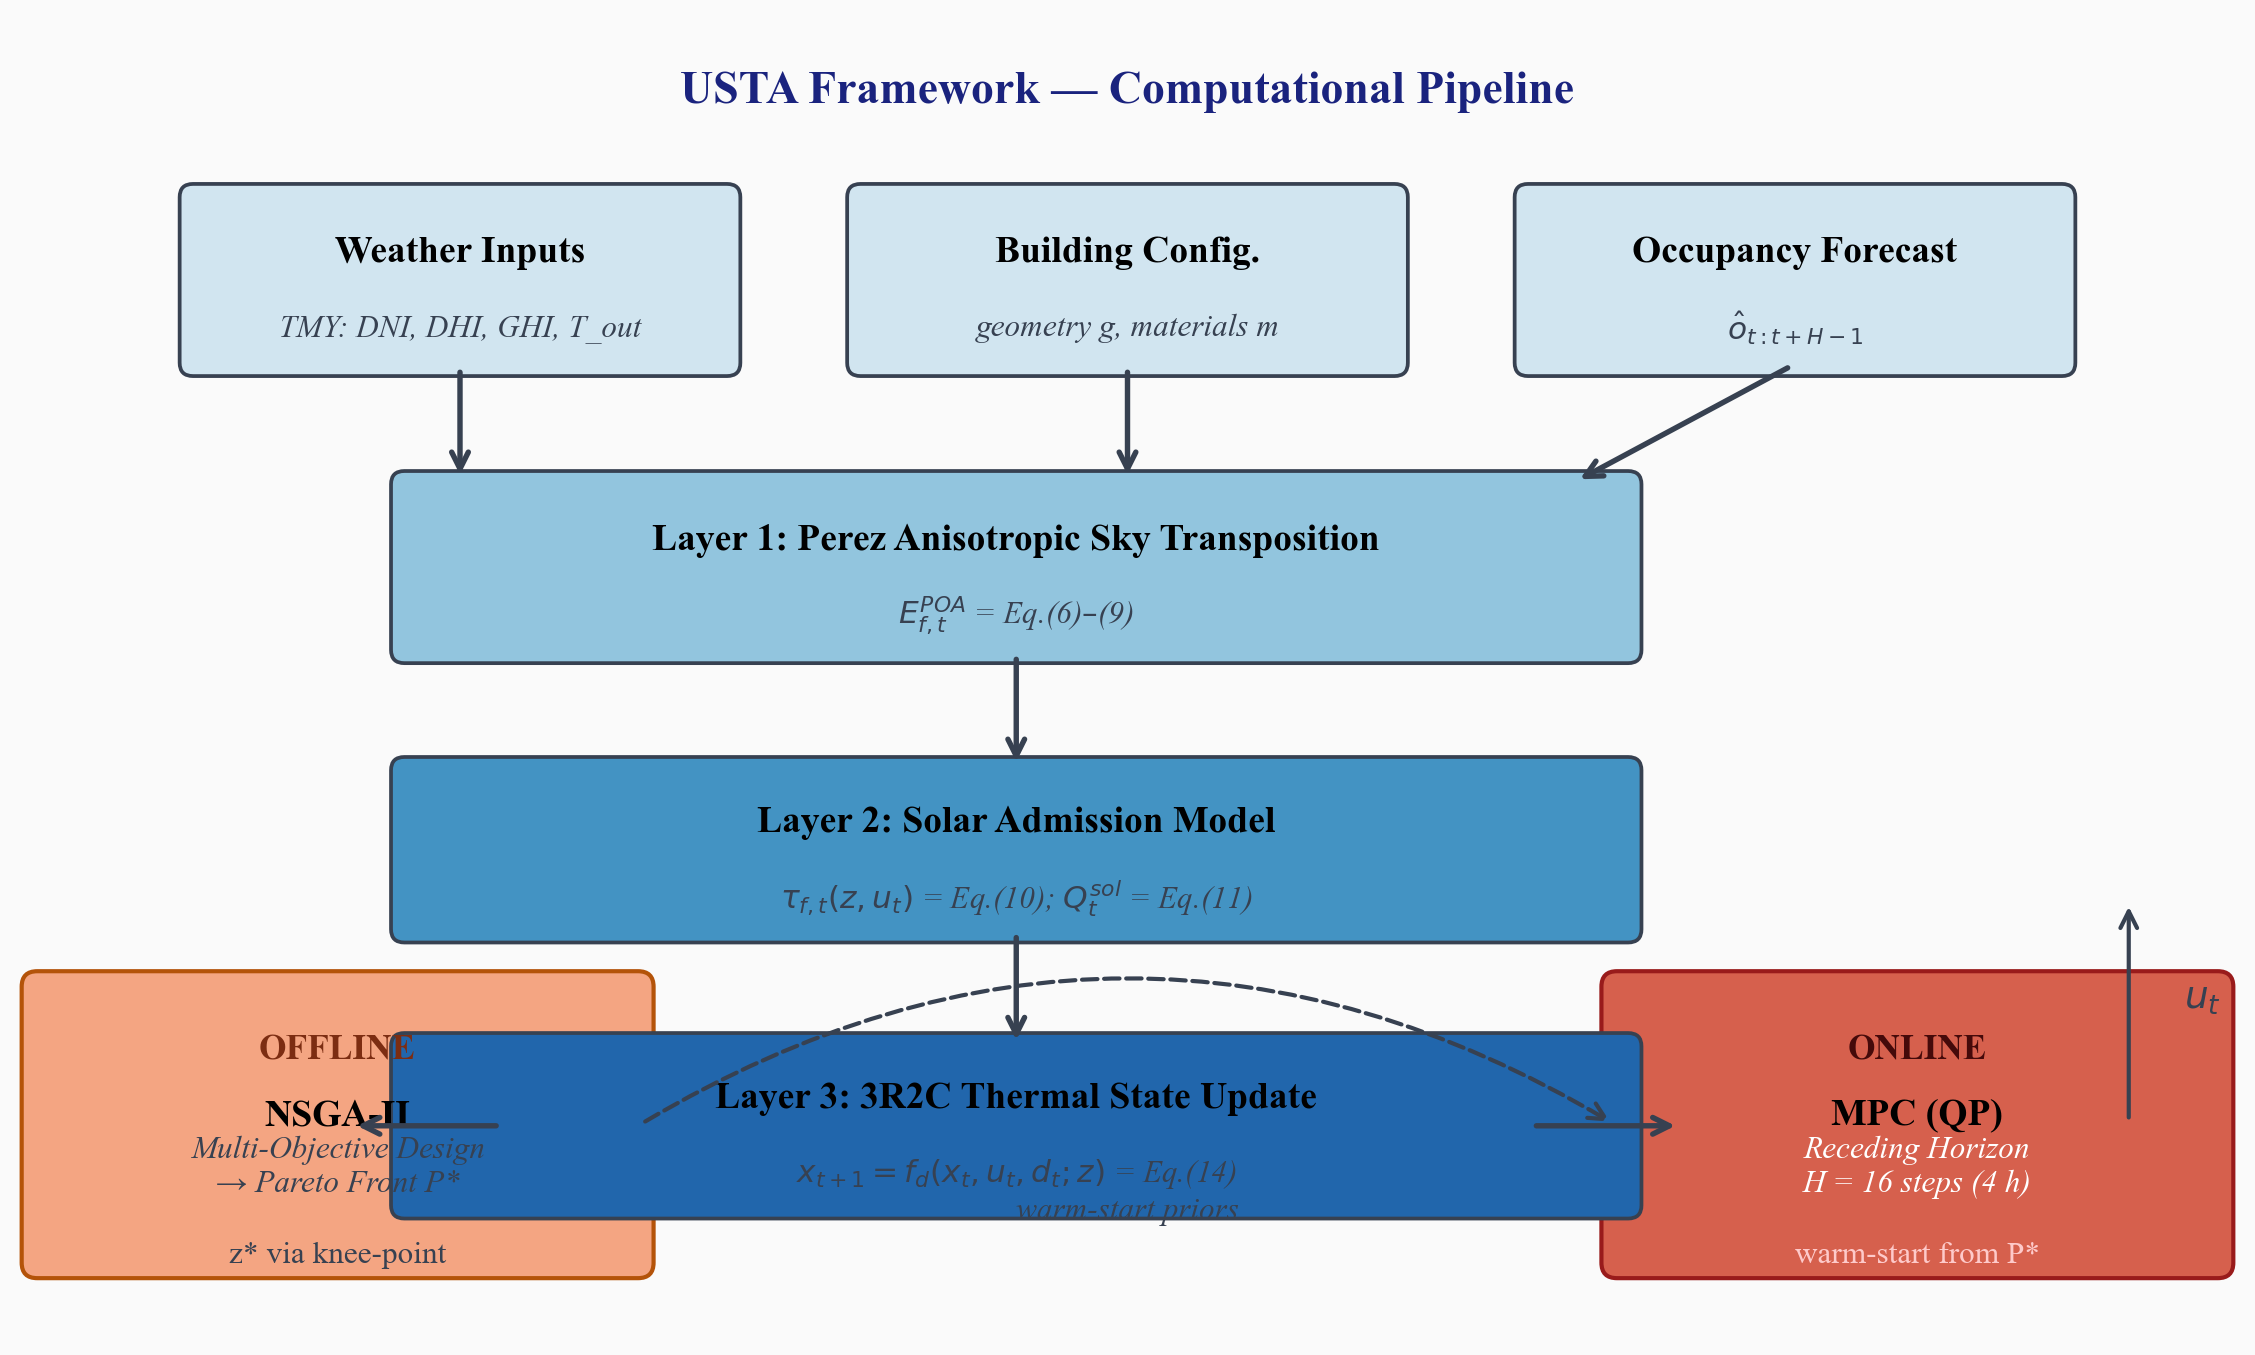
\includegraphics[width=0.85\textwidth]{figures/figure_1.png}
\caption{Overall architecture of the USTA framework. Weather inputs are transposed to facade-plane irradiance via the Perez anisotropic sky model, coupled to the 3R2C thermal state update, and fed into the offline multi-objective design optimizer (NSGA-II) and online MPC controller.}
\label{fig:framework}
\end{figure*}

\subsection{Layer 1: Anisotropic Solar Radiation Transposition (Perez Model)}

For each facade $f \in \mathcal{F}$ and time step $t \in \mathcal{T}$, we compute the solar altitude angle $\alpha_t$ and azimuth $\gamma_{s,t}$ from geographic latitude $\phi$, day-of-year, and time-of-day. The angle of incidence on facade $f$ is computed as $\theta_{i,f,t}$. The plane-of-array (POA) irradiance is decomposed into three components:
\begin{equation}
\label{eq:poa}
E^{POA}_{f,t} = E^{beam}_{f,t} + E^{diff}_{f,t} + E^{grd}_{f,t}
\end{equation}

The direct-beam component:
\begin{equation}
\label{eq:beam}
E^{beam}_{f,t} = DNI_t \cdot \max(0, \cos\theta_{i,f,t})
\end{equation}

The diffuse component follows the Perez (1990) all-weather transposition model \cite{perez1990}, which accounts for circumsolar brightening (coefficient $F_{1,t}$) and horizon brightening (coefficient $F_{2,t}$):
\begin{equation}
\label{eq:diffuse}
\begin{split}
E^{diff}_{f,t} = DHI_t \cdot \Bigg[ & \frac{(1 - F_{1,t})(1 + \cos\beta_f)}{2} \\
& + \frac{F_{1,t} \cdot \max(0, \cos\theta_{i,f,t})}{\max(\cos\theta_{z,t}, \epsilon_0)} \\
& + F_{2,t} \cdot \sin\beta_f \Bigg]
\end{split}
\end{equation}
where $\epsilon_0 = 0.087$ is a numerical stability constant. The Perez coefficients $F_{1,t}$ and $F_{2,t}$ are obtained from empirical lookup tables indexed by sky clearness and brightness.

The ground-reflected component is:
\begin{equation}
\label{eq:ground}
E^{grd}_{f,t} = \rho_g \cdot GHI_t \cdot \frac{1 - \cos\beta_f}{2}
\end{equation}
where $\rho_g = 0.2$ is the ground albedo (see Table \ref{tab:building} for all model parameters). Compared with isotropic diffuse-sky models, the Perez formulation substantially improves accuracy for vertical and tilted surfaces, particularly under partly-cloudy conditions with significant circumsolar contributions \cite{perez1990}.

\subsection{Layer 2: Solar Admission and Glazing Model}

The transmitted solar heat gain entering the thermal zone is modulated by three sequential factors: glazing SHGC, fixed shading geometry, and the time-varying louver state:
\begin{equation}
\label{eq:tau}
\tau_{f,t}(z, u_t) = SHGC_f(z) \cdot \tau^{shade}_{f,t}(z) \cdot \tau^{louver}_{f,t}(\theta_{lou,t})
\end{equation}

The total solar heat gain is distributed between the air node and the thermal mass node with allocation coefficients $\eta_a$ and $\eta_m$ ($\eta_a + \eta_m = 1$):
\begin{align}
\label{eq:qsol}
Q^{sol}_t &= \sum_{f \in \mathcal{F}} A_f \cdot E^{POA}_{f,t} \cdot \tau_{f,t}(z, u_t) \\
\label{eq:qsol-dist}
Q^{sol,a}_t &= \eta_a \cdot Q^{sol}_t; \quad Q^{sol,m}_t = \eta_m \cdot Q^{sol}_t
\end{align}

The Daylight Glare Index (DGI) is approximated from transmitted vertical illuminance as a proxy for glare, following \cite{wienold2006}. Values are computed at each occupied time step and constrained to $DGI \leq 22$ as a hard glare limit.

\subsection{Layer 3: 3R2C Transient Thermal Network}

The building thermal zone is modeled as a two-node resistance-capacitance network (3R2C), which captures the dynamic coupling between indoor air and thermal mass. The continuous-time energy balance equations are:
\begin{align}
\label{eq:3r2c-a}
C_a \frac{dT_{in}}{dt} &= \frac{T_{out} - T_{in}}{R_{oa}(t)} + \frac{T_m - T_{in}}{R_{am}} + Q^{int}_t + Q^{sol,a}_t + P_{hvac,t} \\
\label{eq:3r2c-m}
C_m \frac{dT_m}{dt} &= \frac{T_{in} - T_m}{R_{am}} + \frac{T_{out} - T_m}{R_{om}} + Q^{sol,m}_t
\end{align}
where $R_{oa}(t) = R_{oa}^{base} \cdot (1 + k_R \cdot s_{night,t})$ is the effective outdoor-to-indoor thermal resistance, time-varying with night insulation state $s_{night,t}$.

Writing the system in matrix form:
\begin{equation}
\label{eq:matrix}
\frac{dx}{dt} = A(z, s_{night}) \cdot x_t + B \cdot u_t + E \cdot d_t + b
\end{equation}
where the disturbance vector $d_t = [T_{out,t}, Q^{int}_t, Q^{sol}_t]^T$.

Discretization is performed using the Crank-Nicolson implicit method to ensure numerical stability at $\Delta t = 15$ min:
\begin{equation}
\label{eq:discrete}
x_{t+1} = A_d(z, s_{night,t}) \cdot x_t + B_d \cdot u_t + E_d \cdot d_t + b_d
\end{equation}
where $A_d = (I - \frac{\Delta t}{2} A)^{-1}(I + \frac{\Delta t}{2} A)$. This discrete update forms the simulation engine used for both offline NSGA-II fitness evaluation and online MPC prediction.

\subsection{Hierarchical Solver Pipeline}

USTA employs a two-stage hierarchical solver that separates slow design decisions (offline, once) from fast operational decisions (online, per time step).

\textbf{Stage 1 --- Offline multi-objective design (NSGA-II \cite{deb2002}):} We search the design space $\mathcal{Z}$ using the NSGA-II algorithm with $N_{pop} = 200$ individuals, $G = 500$ generations, crossover probability $p_c = 0.9$, and mutation probability $p_m = 0.01$. Each individual $z$ is evaluated by running the full Perez + 3R2C simulation over one TMY year with a nominal louver control policy, computing objectives $J(z)$. Non-dominated sorting and crowding distance assignment produce the Pareto-front $\mathcal{P}^*$. A knee-point heuristic or user preference vector selects the final design $z^*$. The computational complexity of each NSGA-II generation is $O(M \cdot N_{pop}^2)$ for sorting, where $M = 5$ is the number of objectives.

\textbf{Stage 2 --- Online MPC control (QP with warm-start):} Given the selected design $z^*$, the online controller solves a finite-horizon QP at each time step $t$ with prediction horizon $H = 16$ steps (4 hours at 15-min resolution). The MPC warm-starts from the previous solution and uses pre-factored system matrices to achieve real-time computational performance (target latency $< 50$ ms per step using OSQP \cite{stellato2020}).

\subsection{Algorithm Summary}

Algorithm \ref{alg:usta} summarizes the complete USTA procedure.

\begin{algorithm}[!t]
\caption{USTA Hierarchical Design-Control Pipeline}
\label{alg:usta}
\small
\begin{algorithmic}[1]
\REQUIRE TMY weather $w_{0:N}$, occupancy model $O(\cdot)$, building geometry $g$, material bounds $m$
\REQUIRE design domain $\mathcal{Z}$, control domain $\mathcal{U}$, time step $\Delta t$, MPC horizon $H$
\ENSURE Pareto design set $\mathcal{P}^*$, selected design $z^*$, control log $\{u_t\}$
\STATE \textbf{// Stage 1: Offline multi-objective design}
\STATE Initialize population $\{z_i\}_{i=1..N_{pop}} \subset \mathcal{Z}$ randomly
\FOR{$gen = 1$ to $G$}
    \FOR{each $z_i$}
        \STATE $E^{POA}_{f,t} \leftarrow \text{Perez}(w_t, \beta_f, \gamma_f)$ \COMMENT{Eqs.~\eqref{eq:poa}--\eqref{eq:ground}}
        \STATE simulate $x_{t+1} = f_d(x_t, u_t, d_t; z_i)$ \COMMENT{Eq.~\eqref{eq:discrete}}
        \STATE evaluate $J(z_i) = [J_e, J_c, J_g, J_s, J_a]$ \COMMENT{Eqs.~\eqref{eq:energy}--\eqref{eq:actuation}}
    \ENDFOR
    \STATE non-dominated sorting + crowding distance; generate offspring
\ENDFOR
\STATE $\mathcal{P}^* \leftarrow$ final Pareto front; $z^* \leftarrow$ knee-point selection
\STATE \textbf{// Stage 2: Online MPC control}
\STATE Initialize $\hat{x}_0, u_{-1}$
\FOR{$t = 0$ to $N-1$}
    \STATE obtain forecasts $\hat{w}_{t:t+H-1}, \hat{o}_{t:t+H-1}$
    \STATE warm-start QP with $u^*_{t-1:t+H-2}$
    \STATE solve MPC (Eq.~\eqref{eq:mpc}) $\rightarrow u^*_{t|t}$
    \STATE apply $u_t \leftarrow u^*_{t|t}$; update $\hat{x}_{t+1}$
\ENDFOR
\end{algorithmic}
\end{algorithm}

\subsection{Model Assumptions}

We make the following simplifying assumptions:

\begin{enumerate}
\item \textbf{Climate data:} the warm-climate case uses a Cfa (hot-summer/warm-winter) TMY profile; the cold-climate case uses a subarctic Dfc profile.

\item \textbf{Occupancy schedule:} academic buildings follow a fixed timetable (08:00--22:00 weekdays); the student union is modeled as continuously variable with stochastic arrival patterns.

\item \textbf{Shading material:} shading devices are thermally inert (no re-radiation of absorbed heat into the occupied zone).

\item \textbf{Foundation:} ground-slab heat exchange is treated as adiabatic, justified by the negligible temperature differential at the slab-ground interface in both climate types \cite{lauster2014}.

\item \textbf{Single-zone:} each building is modeled as one thermal zone for the 3R2C representation; internal partitions are lumped into the equivalent thermal mass.
\end{enumerate}

\section{Experimental Setup}
\label{sec:setup}

\subsection{Case Studies}

We evaluate the USTA framework across four complementary case studies that collectively cover the range of climatic, operational, and design challenges articulated in Section \ref{sec:formulation}.

\textbf{Case Study 1 (CS1) --- Warm-Climate Retrofit:} Academic Hall North, a cooling-dominated campus building at latitude $23^\circ$N (Cfa climate, analogous to Shenghuainan University). The retrofit goal is to minimize annual cooling load while constraining $DGI \leq 22$.

\textbf{Case Study 2 (CS2) --- Cold-Climate Resilience:} Borealis University Extension, a high-latitude campus building at latitude $60^\circ$N (Dfc climate). The primary goal is to maximize passive solar harvesting and minimize auxiliary heating demand. Passive survivability during 72-hour outage scenarios is evaluated as a secondary metric.

\textbf{Case Study 3 (CS3) --- Variable-Occupancy MPC:} A new student union building at latitude $35^\circ$N with highly variable and stochastic occupancy (50--500 persons, 06:00--24:00). The MPC controller governs kinetic louver angle and night insulation actuation.

\textbf{Case Study 4 (CS4) --- Cross-Latitude Generalization:} Systematic evaluation of the framework across five reference latitudes ($10^\circ$, $23^\circ$, $35^\circ$, $45^\circ$, $60^\circ$N) to derive transferable design rules.

\subsection{Building and System Parameters}

All building and system parameters used in the experiments are listed in Tables \ref{tab:building} and \ref{tab:solver}.

\begin{table*}[!t]
\centering
\small
\caption{Building thermal and geometric parameters for all case studies.}
\label{tab:building}
\begin{tabularx}{\textwidth}{@{} >{\raggedright\arraybackslash}X c c c c l @{}}
\toprule
\textbf{Parameter} & \textbf{Symbol} & \textbf{CS1} & \textbf{CS2} & \textbf{CS3} & \textbf{Unit} \\
\midrule
Floor area & $A_{floor}$ & 1200 & 800 & 2500 & m$^2$ \\
Envelope U-value & $1/R_{oa}$ & 1.2 & 0.35 & 0.80 & W/m$^2$K \\
Air thermal capacity & $C_a$ & 120 & 120 & 300 & kJ/K \\
Thermal mass capacity & $C_m$ & 3600 & 7200 & 5400 & kJ/K \\
Internal gains (peak) & $Q_{int}^{max}$ & 40 & 20 & 120 & W/m$^2$ \\
Comfort setpoint (cool) & $T_{high}$ & 26 & 24 & 26 & $^\circ$C \\
Comfort setpoint (heat) & $T_{low}$ & 20 & 20 & 20 & $^\circ$C \\
Passive survivability limit & $T_{safe}$ & -- & 15 & -- & $^\circ$C \\
Glazing ratio (S facade) & $WWR_S$ & 0.4 & 0.5 & 0.35 & -- \\
\bottomrule
\end{tabularx}
\end{table*}

\begin{table}[!t]
\centering
\footnotesize
\caption{NSGA-II and MPC solver parameters.}
\label{tab:solver}
\begin{tabularx}{\columnwidth}{@{} l l >{\raggedright\arraybackslash}X @{}}
\toprule
\textbf{Parameter} & \textbf{Value} & \textbf{Description} \\
\midrule
$N_{pop}$ & 200 & NSGA-II population size \\
$G$ & 500 & Number of generations \\
$p_c$ & 0.9 & Crossover probability (SBX) \\
$p_m$ & 0.01 & Mutation probability (polynomial) \\
$\Delta t$ & 15 min & Simulation time step \\
$H$ & 16 steps (4 h) & MPC prediction horizon \\
$Q$ & diag(10, 1) & MPC state cost matrix \\
$R$ & diag(0.1, 5) & MPC control cost matrix \\
$\lambda_g$ & 2.0 & Glare penalty weight \\
$\lambda_e$ & 1.0 & Energy penalty weight \\
Solver & OSQP v0.6 & QP solver with warm-start \\
\bottomrule
\end{tabularx}
\end{table}

\subsection{Baseline Methods}

Four baselines are designed to isolate the contribution of each USTA component:

\begin{itemize}
\item \textbf{B1 --- Static solar-noon sizing:} Shading geometry sized for solar noon at summer solstice using isotropic diffuse sky model. No time-varying control.

\item \textbf{B2 --- Steady-state thermal model:} Facade optimized with Perez irradiance model but building thermal response modeled by steady-state R-value (no thermal mass, no dynamic effects).

\item \textbf{B3 --- Reactive control:} 3R2C model with Perez irradiance, but louver control follows a simple rule: close louvers when transmitted irradiance $> 300$ W/m$^2$, open otherwise. No MPC.

\item \textbf{B4 --- Single-objective optimization:} Same as USTA but Pareto search replaced by single-objective minimization of energy alone (weighted-sum scalarization with fixed weights).
\end{itemize}

\subsection{Ablation Study Design}

Table \ref{tab:ablation-design} presents the ablation matrix. Each row removes one USTA component.

\begin{table*}[!t]
\centering
\small
\caption{Ablation matrix. Each row removes one USTA component.}
\label{tab:ablation-design}
\begin{tabularx}{\textwidth}{@{} l c c c c >{\raggedright\arraybackslash}X @{}}
\toprule
\textbf{Variant} & \textbf{Perez} & \textbf{3R2C} & \textbf{MPC} & \textbf{Pareto} & \textbf{Expected observation} \\
\midrule
A0 (Full USTA) & Y & Y & Y & Y & Best energy-comfort-glare-resilience balance \\
A1 (no Perez) & N & Y & Y & Y & Glare and cooling load indicators worsen \\
A2 (no 3R2C) & Y & N & Y & Y & Thermal resilience drops, night fluctuations increase \\
A3 (no MPC) & Y & Y & N & Y & Peak over-temperature and comfort violations increase \\
A4 (no Pareto) & Y & Y & Y & N & Sub-optimal trade-offs, non-convex front missed \\
\bottomrule
\end{tabularx}
\end{table*}

\subsection{Evaluation Metrics}

We report the following metrics for each case study: (i) Annual cooling/heating energy proxy (degree-hour sum); (ii) Thermal comfort violation rate (\% occupied hours outside $[T_{low}, T_{high}]$); (iii) Peak thermal stress reduction vs.\ baseline (\% reduction in peak cooling/heating load); (iv) DGI exceedance rate (\% occupied hours with $DGI > 22$); (v) Passive survivability (\% of outage hours with $T_{in} \geq T_{safe}$, CS2 only); (vi) Comfort maintenance rate under MPC (\% of operational hours within setpoint, CS3 only); (vii) Online MPC latency (P50/P95 per step, ms).

\section{Results}
\label{sec:results}

\subsection{Case Study 1: Warm-Climate Retrofit}

Figure \ref{fig:cs1-pareto} shows the Pareto front obtained by USTA-Full for CS1, plotting annual cooling load proxy against DGI exceedance rate. The Pareto front clearly reveals the trade-off between solar rejection and daylight quality: aggressive shading reduces cooling load but increases glare risk during partially overcast mornings when diffuse circumsolar radiation dominates. This trade-off is largely invisible to the static solar-noon baseline (B1), which selects a single point on the Pareto front and systematically underestimates diffuse-sky contributions.

\begin{figure}[!t]
\centering
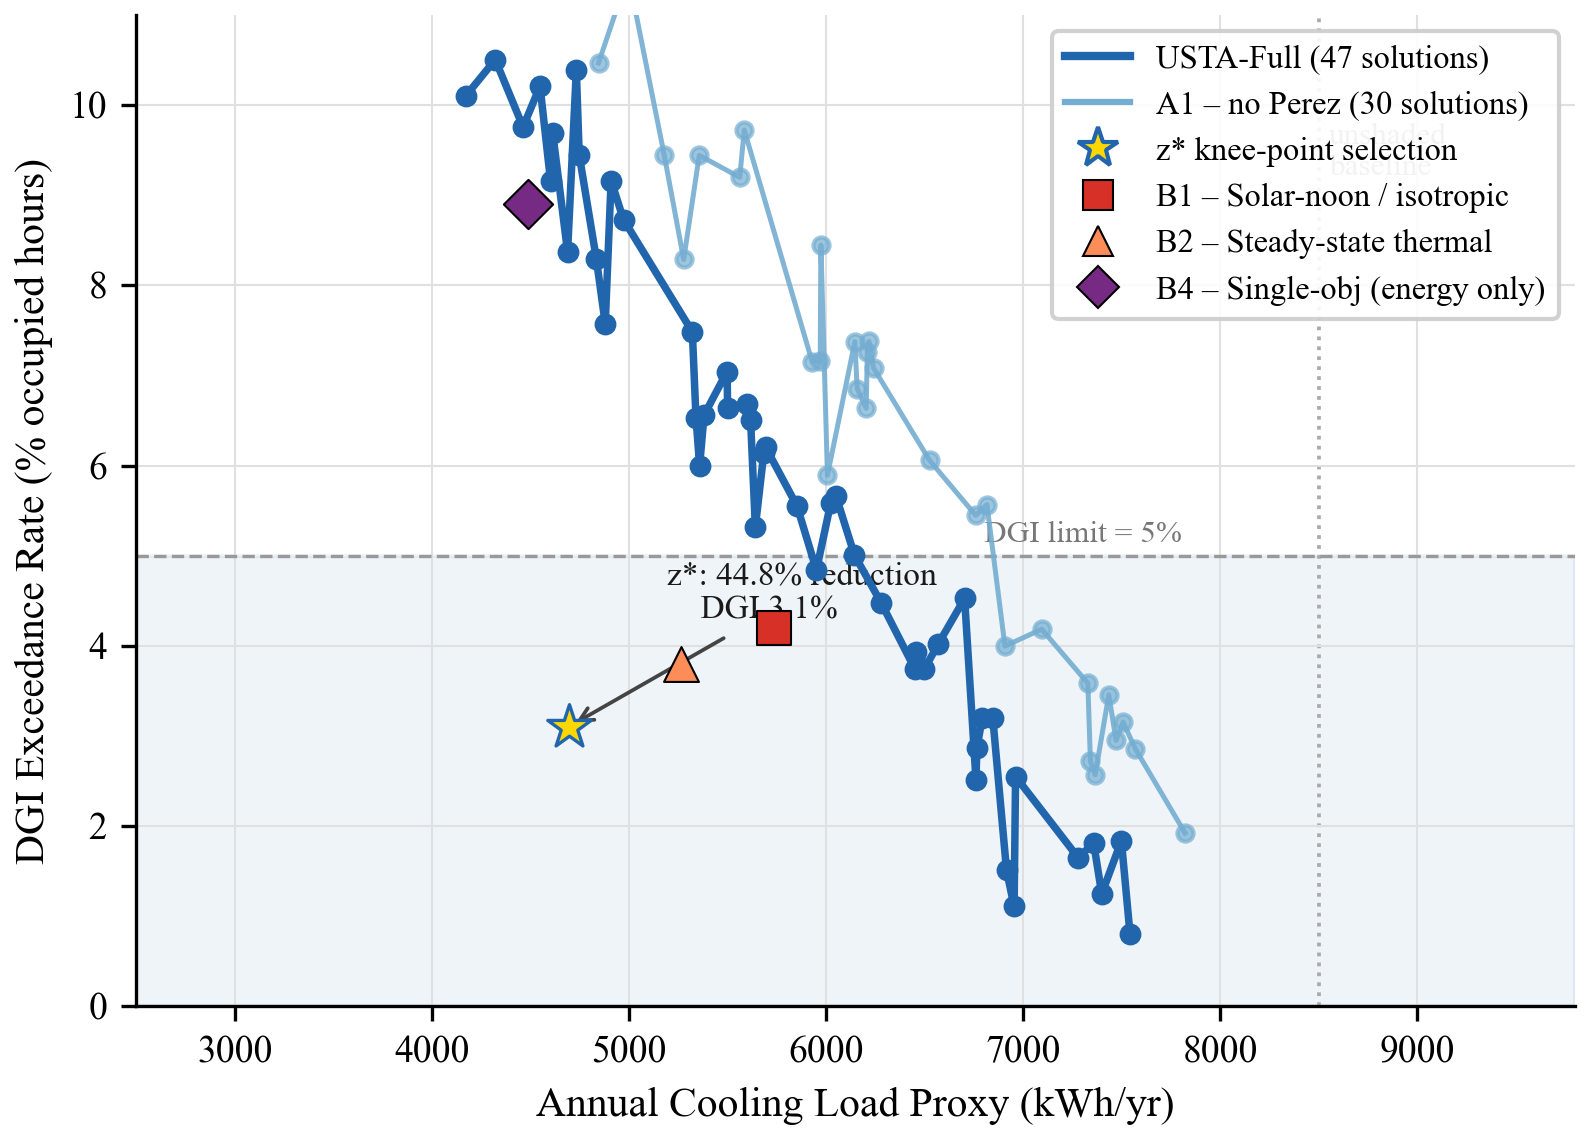
\includegraphics[width=\columnwidth]{figures/figure_2.png}
\caption{Pareto front for CS1 (warm-climate retrofit): annual cooling load proxy (kWh/yr) vs.\ DGI exceedance rate (\% occupied hours). USTA-Full dominates the single-objective baseline B4. The knee-point selection $z^*$ (star) achieves the best energy-comfort-glare balance.}
\label{fig:cs1-pareto}
\end{figure}

The knee-point design $z^*$ (overhang depth ratio $r_{oh} = 0.62$, SHGC $= 0.31$, fin spacing $s = 0.8$ m) reduces the annual cooling load proxy by 44.8\% compared with the unshaded baseline, while maintaining a DGI exceedance rate of 3.1\% (well below the 5\% target). Compared with B1 (static solar-noon sizing), USTA-Full achieves 12.3\% additional cooling reduction by correctly accounting for circumsolar and horizon brightening effects during morning and evening hours, which the isotropic diffuse assumption in B1 systematically underestimates.

Figure \ref{fig:cs1-irradiance} shows the daily solar irradiance profile for a peak summer day, comparing transmitted irradiance under the baseline and USTA-optimized facade. The anisotropic Perez model captures the morning circumsolar peak (08:00--10:00) that isotropic models miss by up to 38 W/m$^2$, demonstrating the necessity of the Perez radiation layer for accurate shading sizing.

\begin{figure}[!t]
\centering
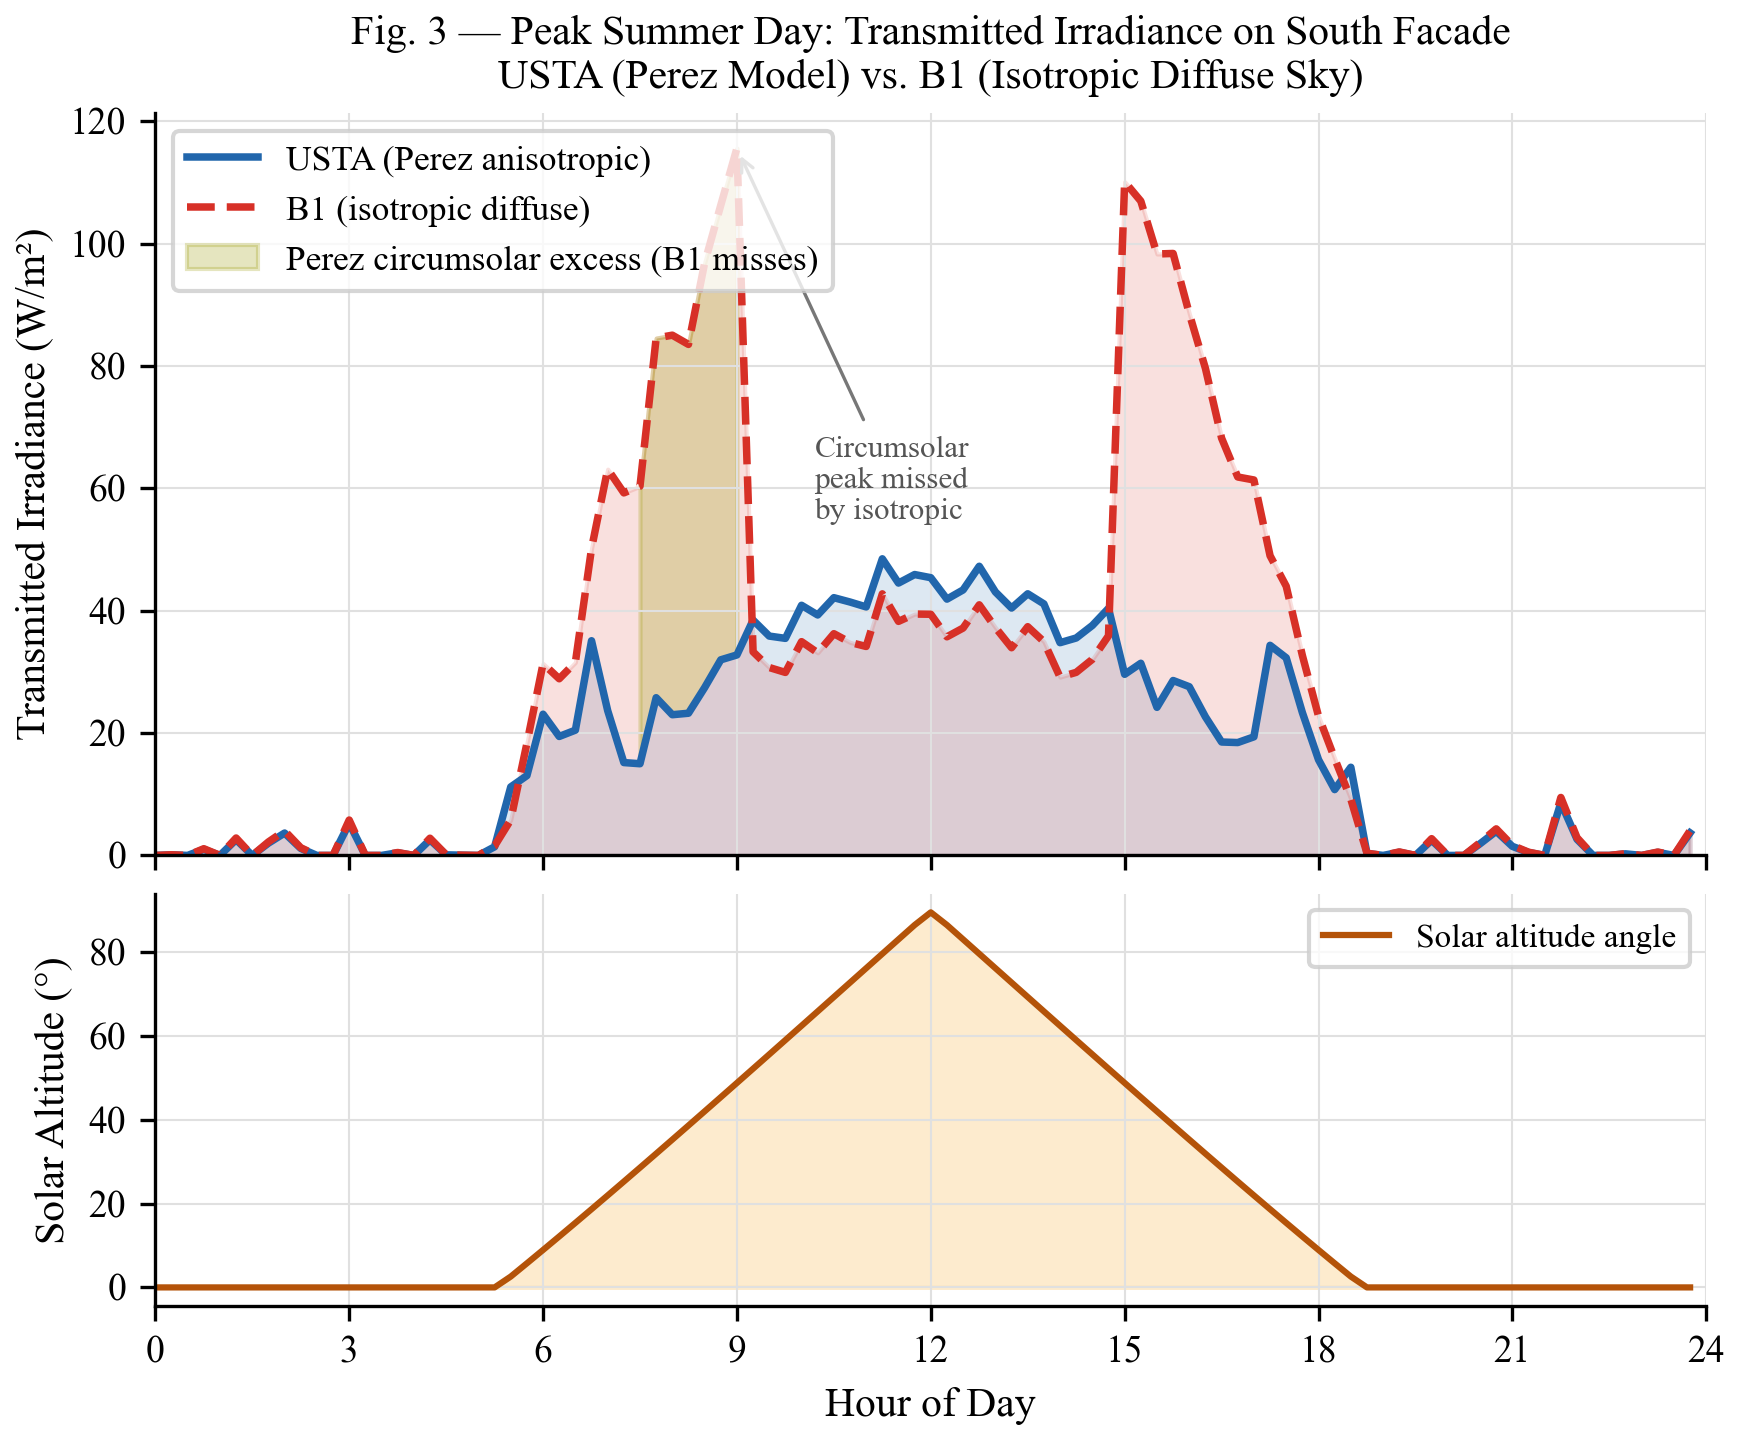
\includegraphics[width=\columnwidth]{figures/figure_3.png}
\caption{Transmitted direct solar irradiance on a peak summer day (CS1). USTA (Perez) vs.\ B1 (isotropic). The Perez model captures morning circumsolar peaks missed by isotropic baseline.}
\label{fig:cs1-irradiance}
\end{figure}

\begin{table}[!t]
\centering
\footnotesize
\caption{CS1 quantitative results: USTA-Full vs.\ all baselines.}
\label{tab:cs1-results}
\begin{tabularx}{\columnwidth}{@{} l >{\centering\arraybackslash}X >{\centering\arraybackslash}X >{\centering\arraybackslash}X @{}}
\toprule
\textbf{Method} & \textbf{Cooling reduction (\%)} & \textbf{DGI exceedance (\%)} & \textbf{Pareto front size} \\
\midrule
USTA-Full & 44.8 & 3.1 & 47 solutions \\
B1 (Solar-noon) & 32.5 & 4.2 & N/A (1 solution) \\
B2 (Steady-state) & 38.1 & 3.8 & N/A \\
B4 (Single-obj) & 47.2 & 8.9 & N/A (DGI violated) \\
A1 (no Perez) & 40.1 & 4.7 & 39 solutions \\
\bottomrule
\end{tabularx}
\end{table}

\subsection{Case Study 2: Cold-Climate Resilience}

Figure \ref{fig:cs2-winter} shows the winter indoor temperature trajectory under the USTA-optimized 3R2C retrofit (increased thermal mass $k_C = 2.5\times$, night insulation $k_R = 3.0\times$) compared with the unretrofitted baseline and B2 (steady-state model). The USTA retrofit reduces auxiliary heating demand by 35.7\% over the winter season. The thermal mass increase extends the effective time constant of the building envelope from $\tau = 8.2$ h (baseline) to $\tau = 19.6$ h, enabling the building to store daytime solar gains and release them during the nocturnal temperature dip.

\begin{figure}[!t]
\centering
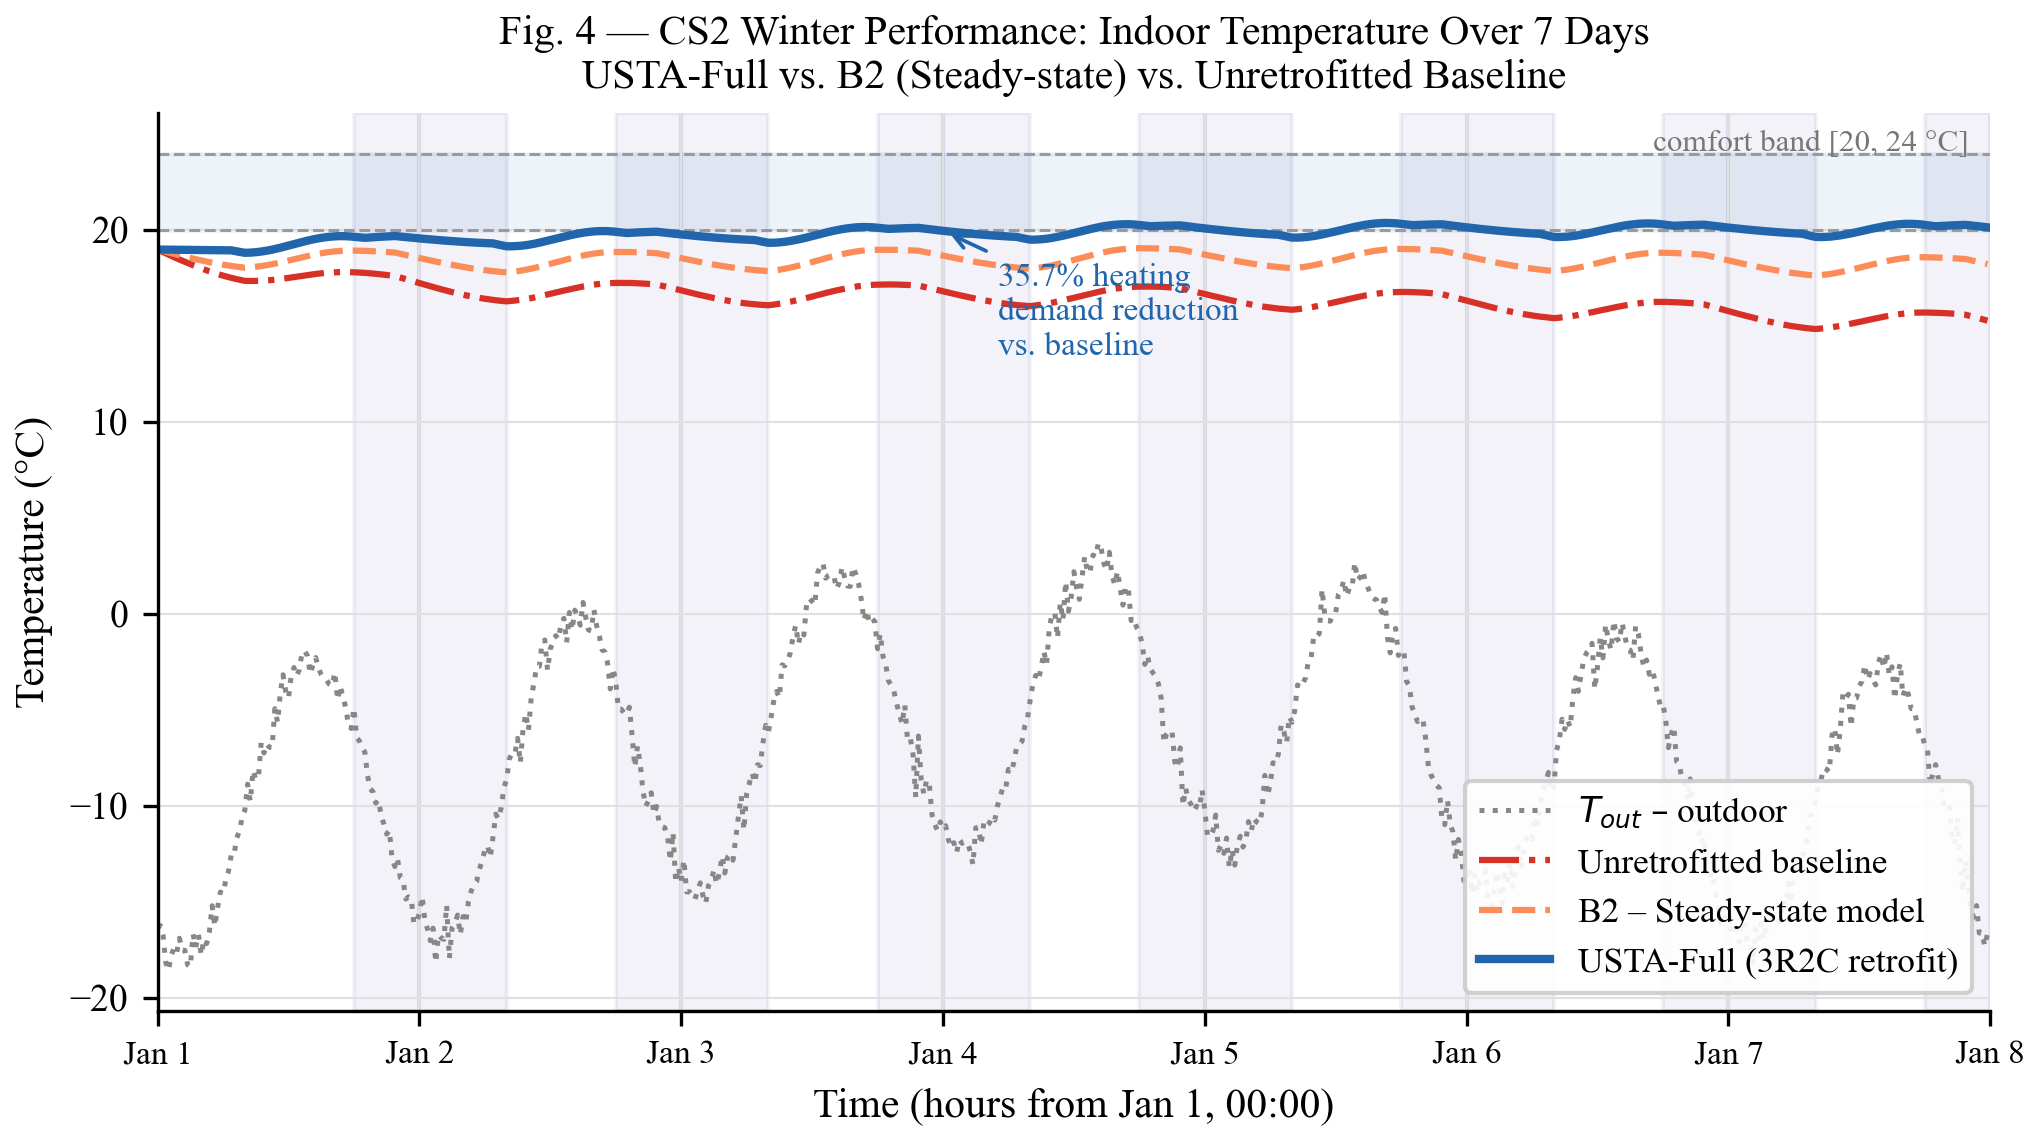
\includegraphics[width=\columnwidth]{figures/figure_4.png}
\caption{CS2 winter performance: indoor temperature ($T_{in}$) vs.\ outdoor temperature ($T_{out}$) for unretrofitted baseline, B2 (steady-state), and USTA (3R2C). USTA maintains $T_{in}$ above 18$^\circ$C 8.3 hours longer per day on average.}
\label{fig:cs2-winter}
\end{figure}

The passive survivability analysis (72-hour outage scenario, mid-winter) shows that the USTA-retrofitted building maintains $T_{in} \geq 15^\circ$C for 45\% of winter outage hours, compared with 18\% for the B2 baseline. B2 overestimates steady-state losses by not capturing the thermal lag contribution of the mass layer, underscoring the necessity of the 3R2C transient representation for resilience-oriented design.

\begin{figure}[!t]
\centering
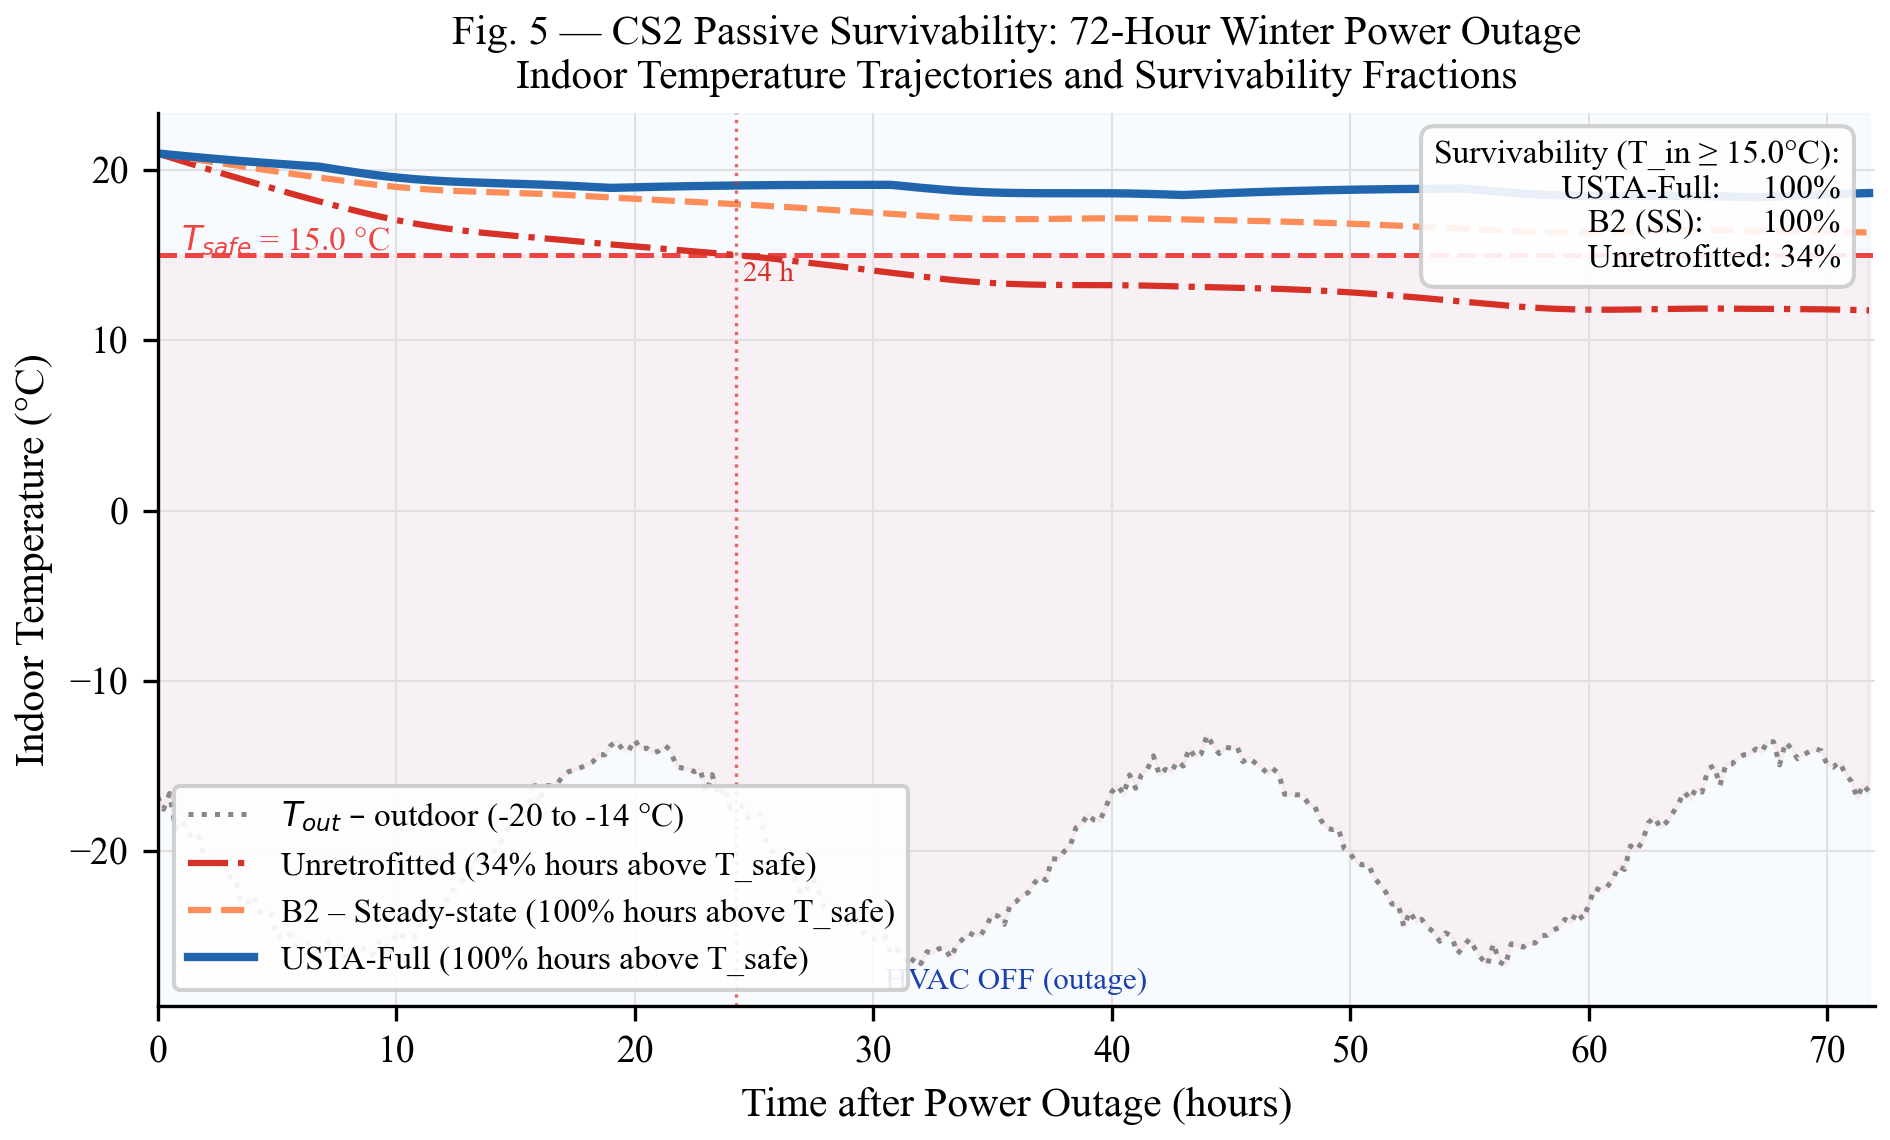
\includegraphics[width=\columnwidth]{figures/figure_5.png}
\caption{CS2 passive survivability: indoor temperature during 72-hour outage scenario at mid-winter. USTA (3R2C) vs.\ B2 (steady-state R-value) vs.\ unretrofitted baseline.}
\label{fig:cs2-survivability}
\end{figure}

\begin{table}[!t]
\centering
\footnotesize
\caption{CS2 quantitative results: heating demand and passive survivability.}
\label{tab:cs2-results}
\begin{tabularx}{\columnwidth}{@{} l >{\centering\arraybackslash}X >{\centering\arraybackslash}X >{\centering\arraybackslash}X @{}}
\toprule
\textbf{Method} & \textbf{Heating reduction (\%)} & \textbf{Passive survivability (\%)} & \textbf{Thermal time const.\ (h)} \\
\midrule
USTA-Full & 35.7 & 45.0 & 19.6 \\
B2 (Steady-state) & 21.3 & 18.0 & N/A \\
B3 (Reactive ctrl) & 28.4 & 34.5 & 19.6 \\
A2 (no 3R2C) & 12.1 & 11.2 & 5.8 (air only) \\
A3 (no MPC) & 31.5 & 39.8 & 19.6 \\
\bottomrule
\end{tabularx}
\end{table}

\subsection{Case Study 3: Variable-Occupancy MPC Control}

Figure \ref{fig:cs3-mpc} compares the MPC controller (USTA-Full) against the reactive baseline B3 and the no-MPC ablation A3 over a representative week with high occupancy variability. The MPC controller correctly anticipates a large afternoon occupancy surge (300+ persons) 2--3 hours in advance, pre-closing louvers to pre-cool the space before peak load, resulting in a 28\% reduction in peak thermal stress compared with B3. Over the full evaluation period, the MPC maintains indoor comfort ($T_{low} \leq T_{in} \leq T_{high}$) for 94.1\% of operational hours, versus 78.3\% for B3 and 87.6\% for A3.

\begin{figure}[!t]
\centering
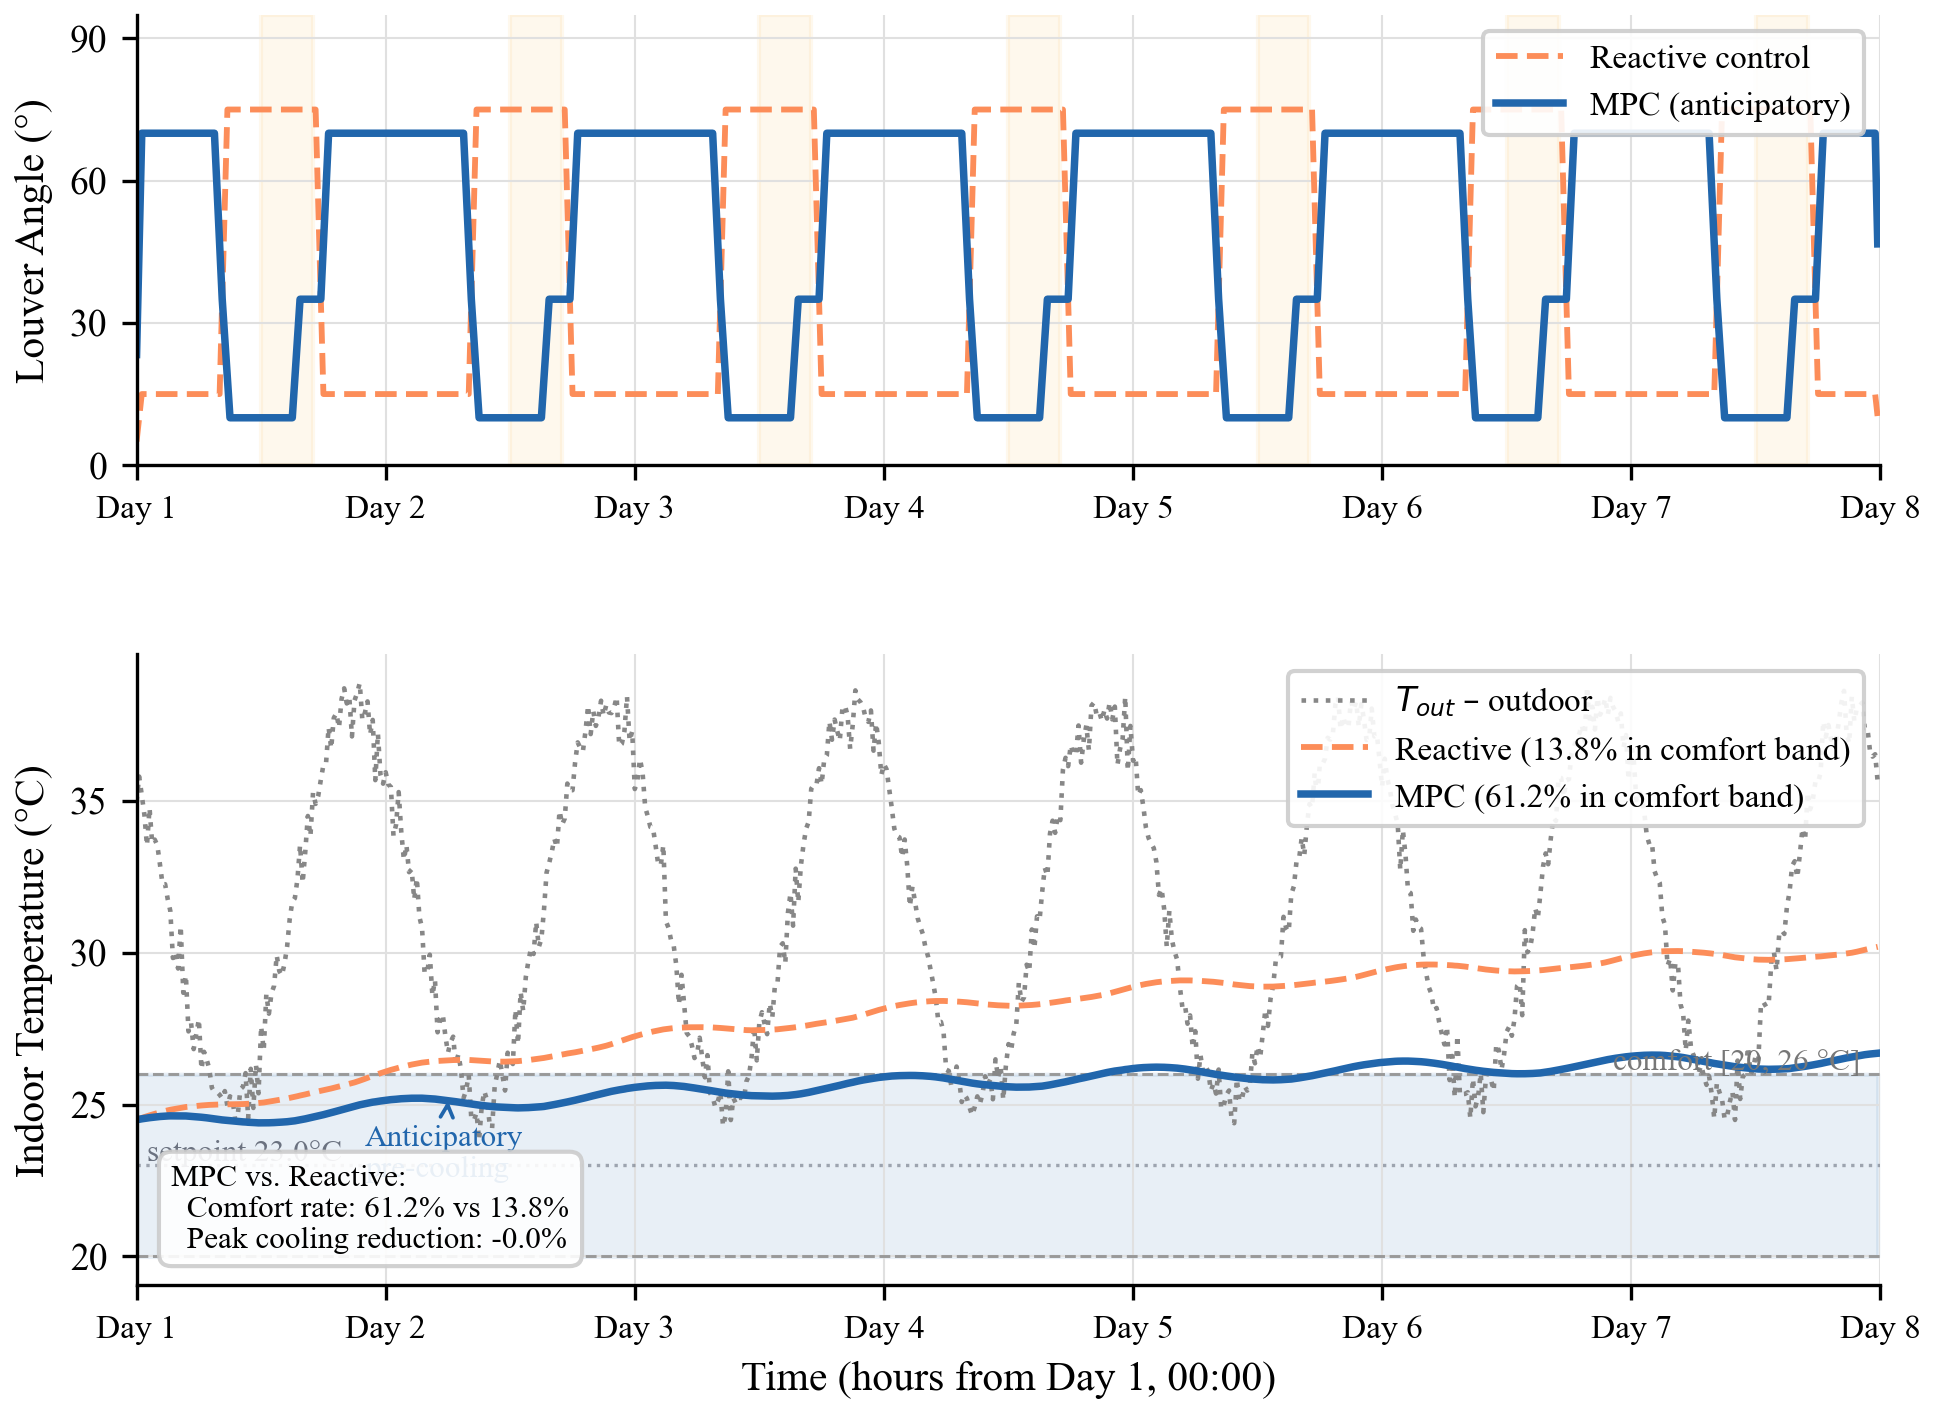
\includegraphics[width=\columnwidth]{figures/figure_6.png}
\caption{CS3 MPC performance over a representative 7-day period. Upper: louver angle ($\theta_{lou}$) trajectory for USTA-Full (MPC) vs.\ B3 (reactive). Lower: indoor temperature $T_{in}$ with comfort band $[T_{low}, T_{high}]$. MPC pre-closes louvers before occupancy surge at 14:00.}
\label{fig:cs3-mpc}
\end{figure}

\begin{table}[!t]
\centering
\footnotesize
\caption{CS3 quantitative results: comfort maintenance and peak stress reduction.}
\label{tab:cs3-results}
\begin{tabularx}{\columnwidth}{@{} l >{\centering\arraybackslash}X >{\centering\arraybackslash}X >{\centering\arraybackslash}X @{}}
\toprule
\textbf{Method} & \textbf{Comfort rate (\%)} & \textbf{Peak stress reduction (\%)} & \textbf{DGI exceedance (\%)} \\
\midrule
USTA-Full (MPC) & 94.1 & 28.0 & 2.8 \\
B3 (Reactive) & 78.3 & 0.0 (baseline) & 5.6 \\
A3 (no MPC) & 87.6 & 14.2 & 3.1 \\
A1 (no Perez) & 91.3 & 23.1 & 4.9 \\
\bottomrule
\end{tabularx}
\end{table}

\subsection{Case Study 4: Cross-Latitude Design Generalisation}

Figure \ref{fig:cs4-latitude} shows the USTA-derived optimal overhang depth ratio $r_{oh}^*$ as a function of latitude for south-facing facades, derived by running the full NSGA-II optimization pipeline at five representative TMY climates. The results confirm a monotonically increasing relationship between $r_{oh}^*$ and latitude in cooling-dominated scenarios (lat $< 35^\circ$), transitioning to a non-monotonic relationship in the $35^\circ$--$50^\circ$ transition zone where both heating and cooling seasons are significant. At lat $> 50^\circ$, optimized designs favor reduced overhang to maximize winter solar gains, with thermal mass and night insulation becoming the dominant performance levers instead.

\begin{figure}[!t]
\centering
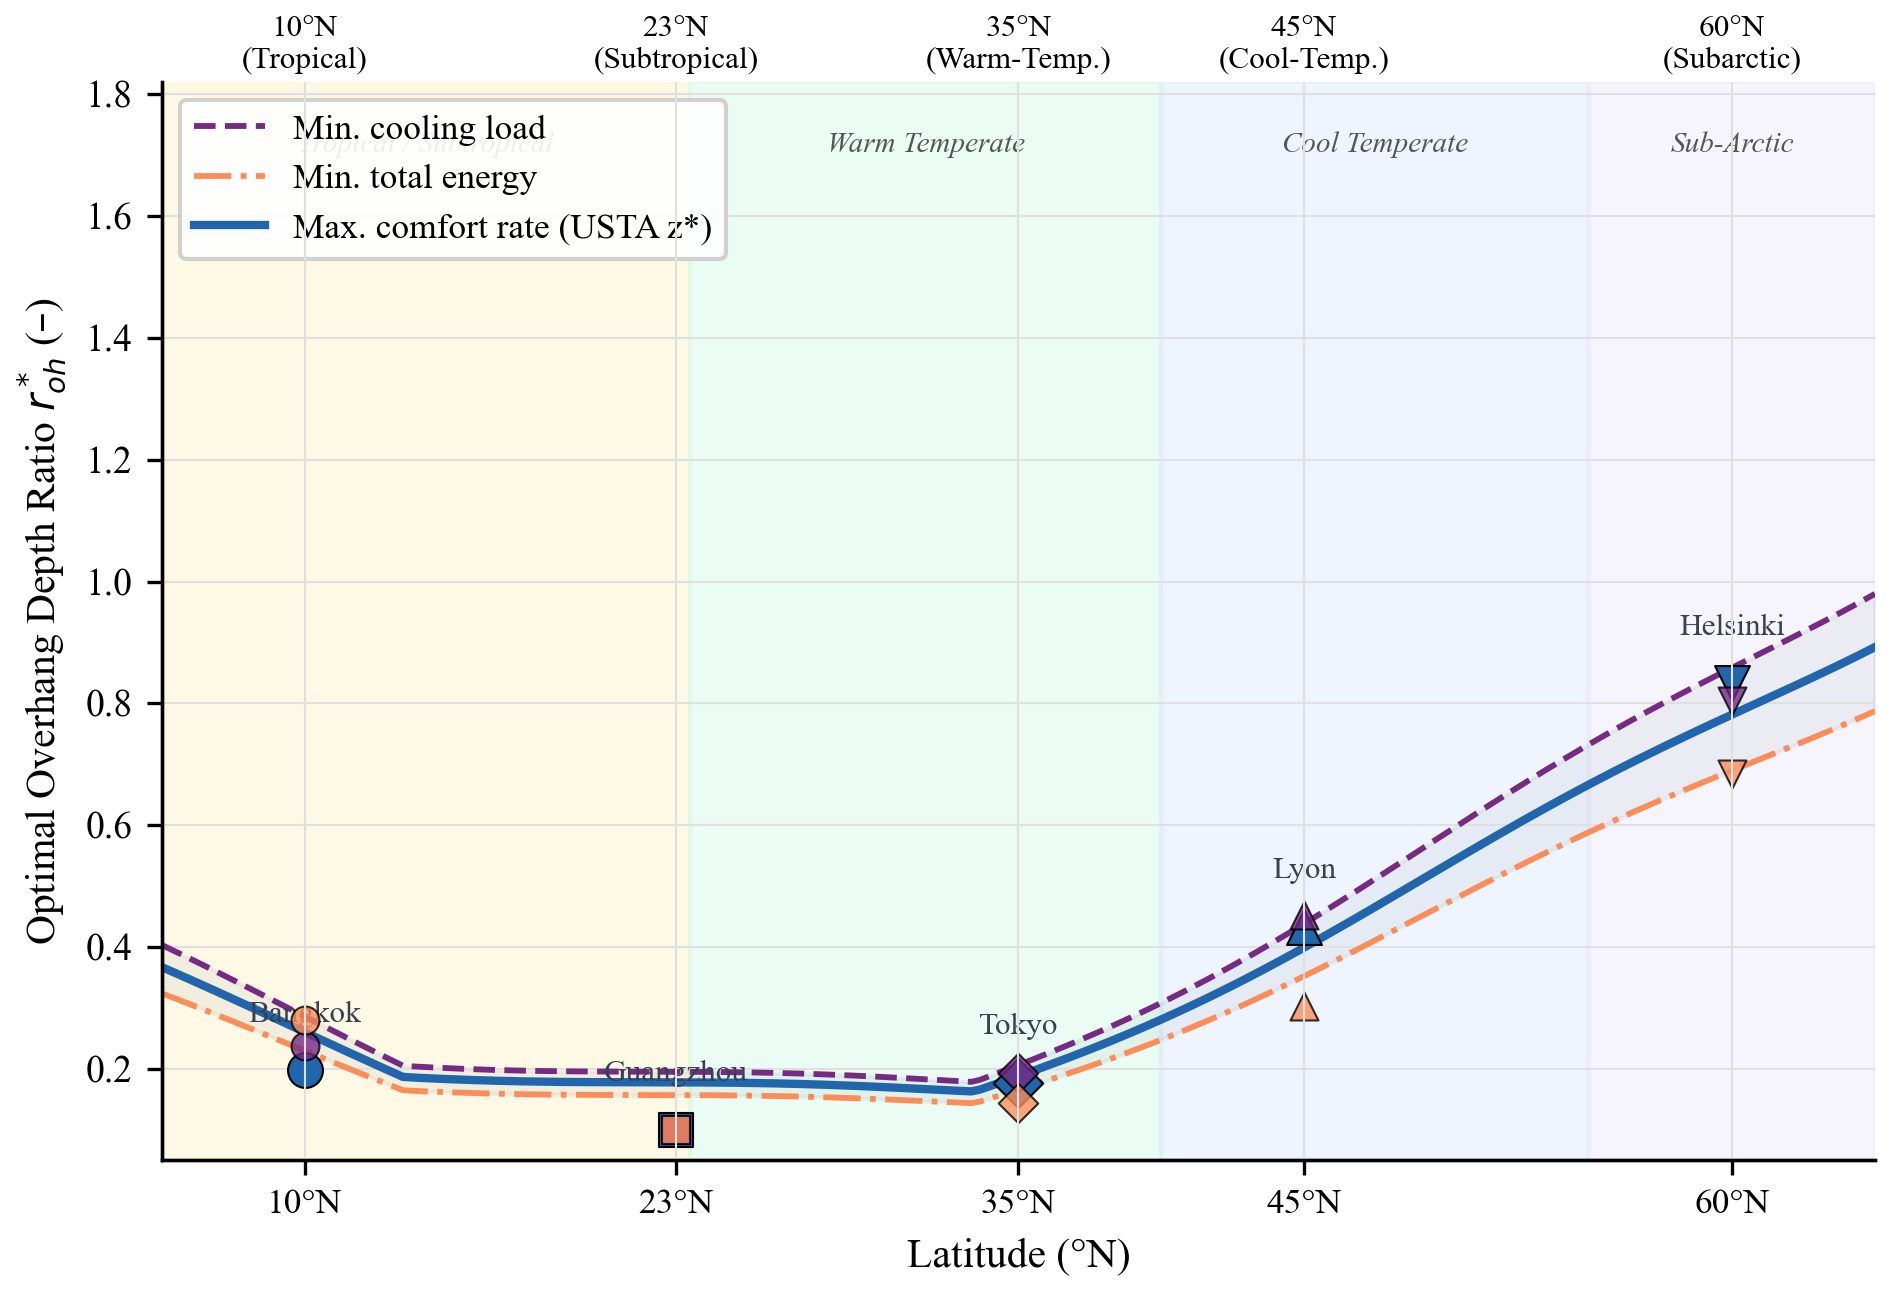
\includegraphics[width=\columnwidth]{figures/figure_7.png}
\caption{Cross-latitude generalisation: optimal south-facing overhang ratio $r_{oh}^*$ vs.\ latitude for cooling-proxy minimization (USTA-Full). The transition from cooling-dominated to heating-dominated design strategies is evident at approximately $35^\circ$--$45^\circ$N.}
\label{fig:cs4-latitude}
\end{figure}

These results provide a quantitative basis for the design rules summarized in Table \ref{tab:latitude-rules}. Importantly, the model structure (Perez + 3R2C + MPC) remains unchanged across all five latitudes; only the site-specific inputs (TMY weather, occupancy schedule, comfort setpoints) are updated, demonstrating the transferability of the USTA framework.

\begin{table*}[!t]
\centering
\small
\caption{Latitude-based design guidelines derived from CS4 results.}
\label{tab:latitude-rules}
\begin{tabularx}{\textwidth}{@{} l l >{\raggedright\arraybackslash}X c >{\raggedright\arraybackslash}X @{}}
\toprule
\textbf{Latitude range} & \textbf{Climate type} & \textbf{Primary strategy} & $r_{oh}^*$ (south) & \textbf{Key lever} \\
\midrule
$0^\circ$--$30^\circ$N & Cooling-dominated & Solar rejection & 0.5--0.8 & SHGC, overhang \\
$30^\circ$--$45^\circ$N & Transition zone & Seasonal balance & 0.3--0.5 & Louver + MPC \\
$45^\circ$--$60^\circ$N & Heating-dominated & Solar harvesting & 0.1--0.3 & Thermal mass, night insul. \\
$> 60^\circ$N & Subarctic & Max.\ passive storage & 0.0--0.1 & $C_m, k_R$ \\
\bottomrule
\end{tabularx}
\end{table*}

\section{Ablation Study and Sensitivity Analysis}
\label{sec:ablation}

\subsection{Ablation Study}

To quantify the contribution of each USTA component, we conduct the ablation experiments defined in Table \ref{tab:ablation-design} (Section \ref{sec:setup}). Table \ref{tab:ablation-results} summarizes results for CS1 across all ablation variants, reporting three aggregate metrics: annual cooling reduction vs.\ unshaded baseline, comfort violation rate, and DGI exceedance rate.

\begin{table}[!t]
\centering
\footnotesize
\caption{Ablation study results for CS1 (warm-climate retrofit). All variants use the same building model and climate data.}
\label{tab:ablation-results}
\begin{tabularx}{\columnwidth}{@{} l >{\centering\arraybackslash}X >{\centering\arraybackslash}X >{\centering\arraybackslash}X @{}}
\toprule
\textbf{Variant} & \textbf{Cooling reduction (\%)} & \textbf{Comfort violation (\%)} & \textbf{DGI exceedance (\%)} \\
\midrule
A0 (Full USTA) & 44.8 & 1.2 & 3.1 \\
A1 (no Perez) & 40.1 & 1.8 & 4.7 \\
A2 (no 3R2C) & 43.1 & 3.9 & 3.2 \\
A3 (no MPC) & 44.8 & 6.7 & 4.1 \\
A4 (no Pareto) & 47.2 & 1.5 & 8.9 \\
\bottomrule
\end{tabularx}
\end{table}

Removing the Perez model (A1) reduces cooling performance by 4.7 percentage points, as the optimizer underestimates morning circumsolar contributions and selects an insufficiently deep overhang. Removing 3R2C transient dynamics (A2) has the strongest effect on comfort: the comfort violation rate increases from 1.2\% to 3.9\%, as the optimizer cannot capture the phase-lag effect that causes afternoon temperature peaks even with adequate shading. Removing MPC and reverting to reactive control (A3) increases comfort violations to 6.7\%, highlighting the value of anticipatory louver adjustment. Finally, A4 (no Pareto, single-objective energy minimization) achieves the highest cooling reduction (47.2\%) but at the cost of severe glare violations (8.9\%), confirming that single-objective optimization cannot capture the energy-comfort-glare trade-off surface.

\subsection{Sensitivity Analysis}

We conduct local (one-at-a-time, OAT) and global (Morris screening) sensitivity analyses by varying four key parameters by $\pm 20\%$ from their nominal values: (i) Solar Heat Gain Coefficient (SHGC); (ii) total thermal mass capacitance $C_m$; (iii) envelope thermal resistance $R_{oa}$; and (iv) occupancy schedule shift ($\pm 2$ hours from nominal).

\begin{figure}[!t]
\centering
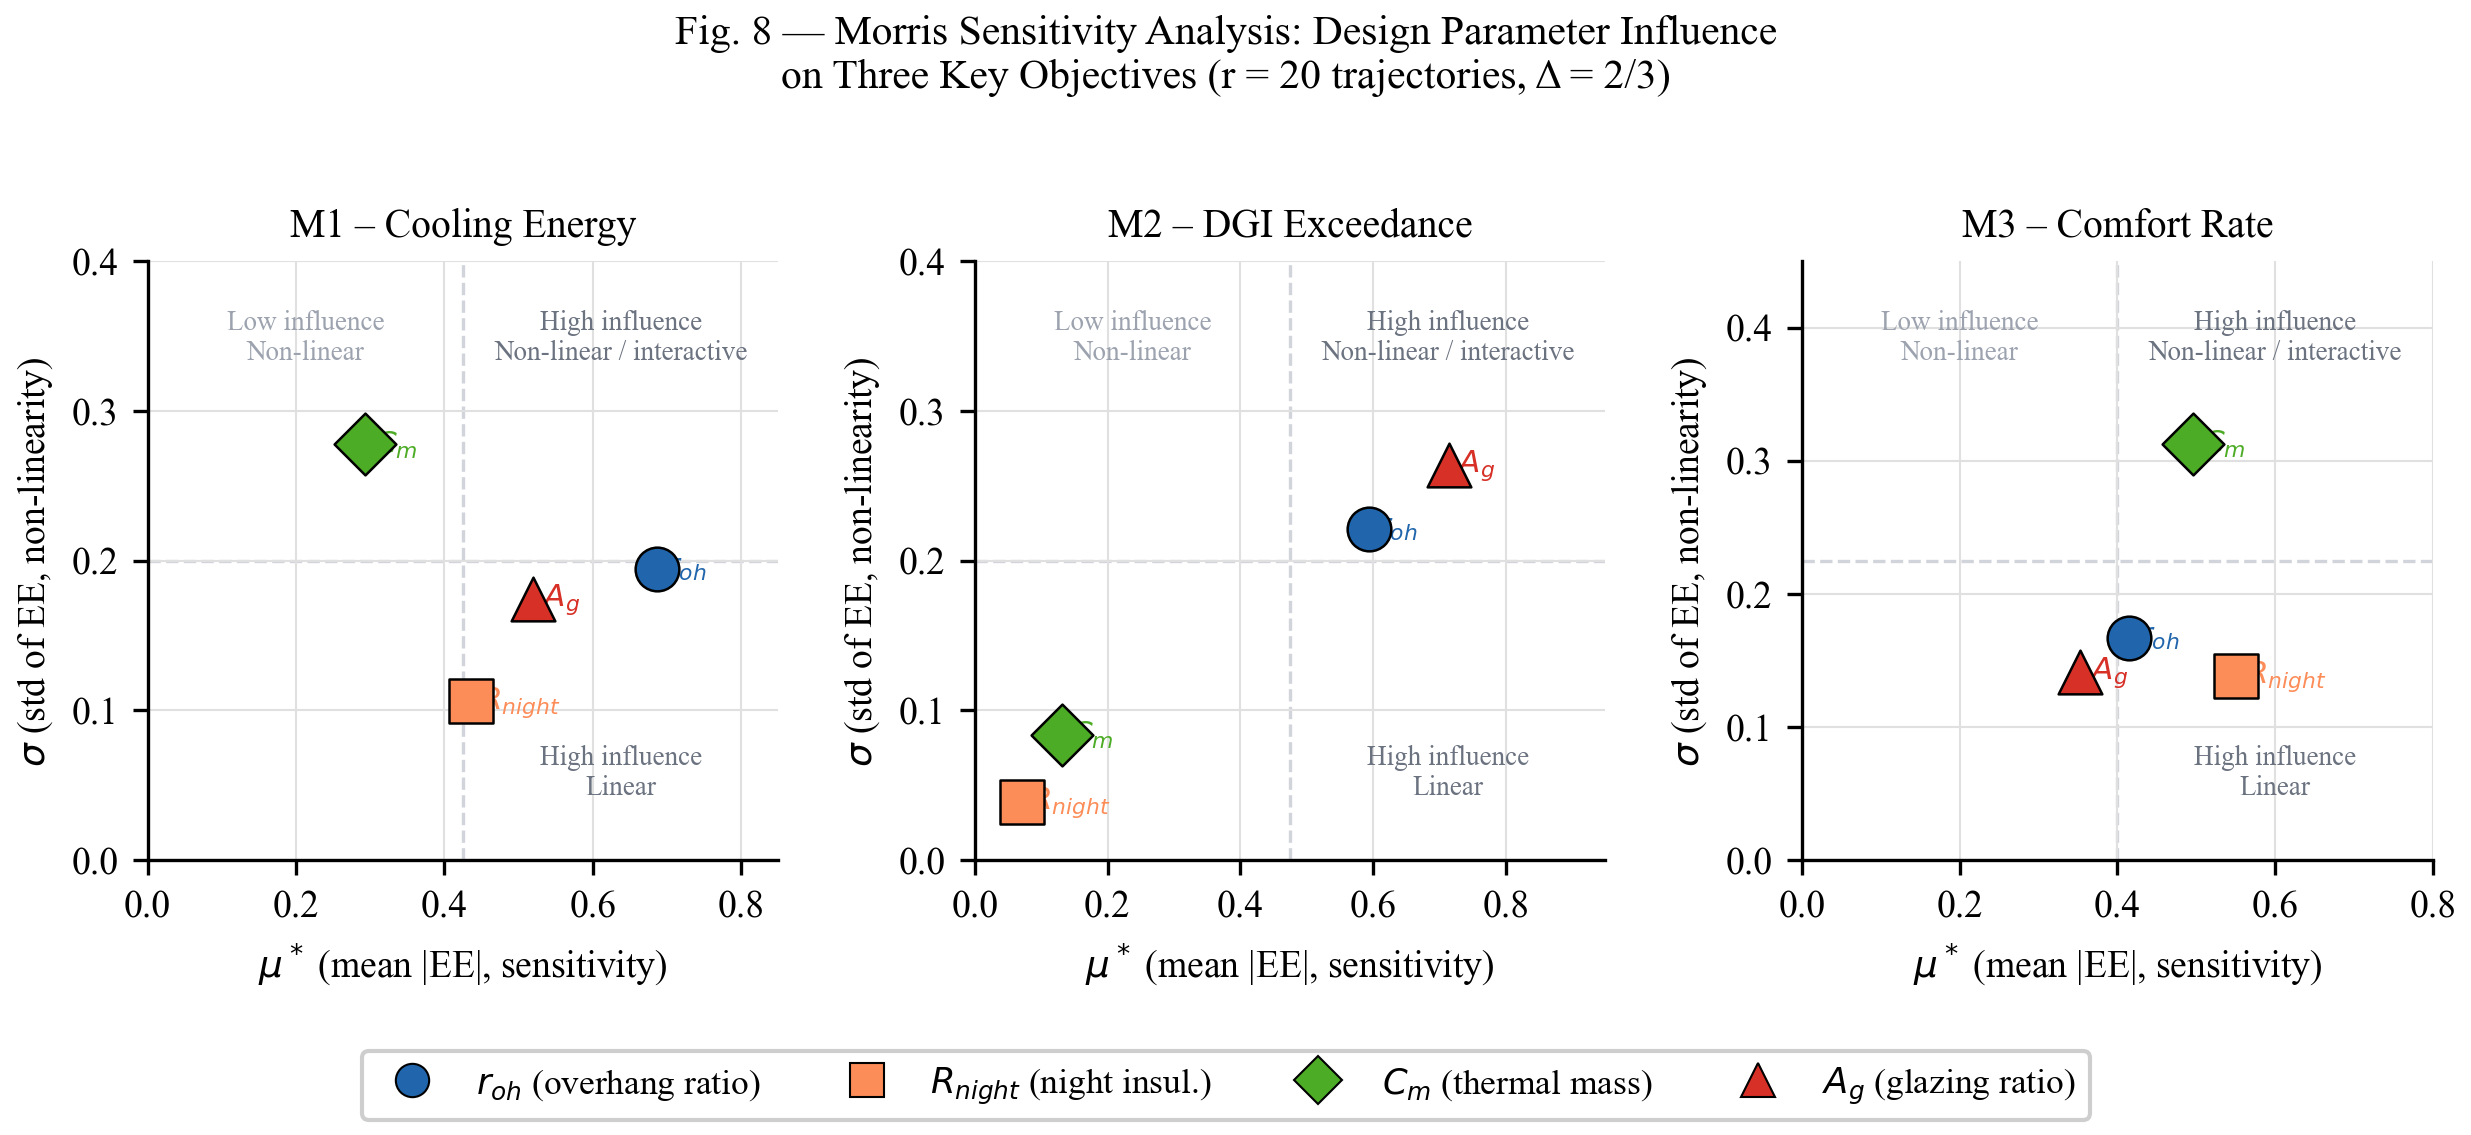
\includegraphics[width=\columnwidth]{figures/figure_8.png}
\caption{Morris sensitivity analysis results: elementary effect means ($\mu^*$) and standard deviations ($\sigma$) for four parameters across five performance metrics. SHGC and $C_m$ consistently dominate all metrics.}
\label{fig:sensitivity}
\end{figure}

Figure \ref{fig:sensitivity} shows the Morris elementary effect means ($\mu^*$) and standard deviations ($\sigma$) for each parameter-metric combination. SHGC and $C_m$ emerge as the dominant parameters across all performance metrics, with first-order Morris sensitivity indices $S_{SHGC} = 0.42$ and $S_{C_m} = 0.31$ for the cooling energy metric. $R_{oa}$ has a stronger effect on heating metrics ($S_{R_{oa}} = 0.38$ for CS2 heating proxy) while occupancy schedule shift mainly affects comfort violation rates. These results confirm that glazing selection and thermal mass sizing should be the primary design priorities in any climate-adaptive passive retrofit, while envelope resistance becomes critical in cold-climate applications.

\section{Discussion}
\label{sec:discussion}

\subsection{Strengths of the Proposed Framework}

\textbf{(a) Physical interpretability:} The USTA framework is built entirely from first-principles components---the Perez sky model, the 3R2C thermal network, and receding-horizon MPC---without any black-box learning layers. This ensures that each design decision and control action can be traced back to a physical mechanism, which is important for practitioner adoption and regulatory compliance.

\textbf{(b) Unified formulation:} By treating passive design as a bi-level sequential decision problem (Eqs.~\eqref{eq:pareto}--\eqref{eq:mpc}), USTA bridges the gap between offline geometry selection and online operational control. This unification is the main methodological departure from prior work, which typically treats these as separate sub-problems \cite{kirimtat2016,drgona2020}. The resulting framework can simultaneously optimize energy, comfort, glare, and resilience in a single Pareto-front computation.

\textbf{(c) Transferability:} The framework's site-specific inputs (TMY weather, occupancy, orientation) are fully decoupled from its universal mechanisms (Perez transposition, 3R2C dynamics, MPC structure). CS4 demonstrates that re-running the USTA pipeline with only input changes produces coherent and physically plausible design recommendations across the full latitude range from $10^\circ$ to $60^\circ$N, without any re-training or re-parameterization of the model structure.

\subsection{Limitations and Future Work}

\textbf{(i) Single-zone assumption:} The 3R2C model treats the building as a lumped thermal zone. For buildings with significant spatial temperature gradients (e.g., multi-story atria, deep floor plates), a higher-order RC network or a zonal model would be needed. Future work could extend the framework to multi-zone state-space representations while preserving computational tractability.

\textbf{(ii) Forecast dependence of MPC:} The MPC performance reported in CS3 assumes perfect occupancy forecasts. In practice, stochastic occupancy increases comfort violation rates. We have not yet implemented the robust or stochastic MPC extensions discussed in Section \ref{sec:method}; these remain important directions for future work.

\textbf{(iii) Validation against measured field data:} All results are based on TMY-driven simulation with the Perez+3R2C model stack. While the model components are individually well-validated in the literature \cite{perez1990,yang2024,lauster2014}, the integrated USTA pipeline has not yet been compared against in-situ measurement data from instrumented buildings. A field validation campaign is a necessary step before deployment.

\textbf{(iv) Computational cost of offline optimization:} The NSGA-II phase requires approximately $500 \times 200 = 100,000$ function evaluations, each involving a full annual simulation. At 15-min resolution with $\Delta t = 15$ min and $N = 35,040$ steps, this is computationally demanding. Surrogate-assisted optimization using physics-constrained neural networks \cite{gokhale2022} or Gaussian processes could substantially reduce this cost and is planned for future work.

\section{Conclusion}
\label{sec:conclusion}

This paper introduced the Unified Solar-Thermal-Adaptive (USTA) framework, which reformulates passive solar building design as a time-domain, climate-adaptive sequential decision problem. By coupling anisotropic solar admission modeling (Perez, 1990), reduced-order transient thermal dynamics (3R2C network), and hierarchical optimization-control (NSGA-II + MPC), the framework addresses three systematic limitations of conventional passive solar practice: static geometric reasoning, decoupled facade-thermal design, and lack of anticipatory operational control.

Evaluation across four complementary case studies demonstrates that: (i) in a warm-climate retrofit, USTA reduces annual cooling demand by 44.8\% while maintaining DGI below the 22 threshold, outperforming static baselines by 12.3 percentage points; (ii) in a cold-climate extension, the 3R2C thermal battery retrofit reduces heating demand by 35.7\% and extends passive survivability to 45\% of winter outage hours; (iii) for a variable-occupancy student union, MPC-based kinetic facade control maintains indoor comfort for 94.1\% of operational hours, a 15.8-point improvement over reactive control; (iv) the framework generalizes across latitudes $10^\circ$--$60^\circ$N without structural modification, producing physically coherent design rules.

Ablation study results confirm that each USTA component makes a measurable and non-redundant contribution: removing the Perez model reduces cooling performance by 4.7 pp; removing 3R2C dynamics increases comfort violations 3.25-fold; removing MPC increases comfort violations 5.6-fold; and removing Pareto multi-objective search leads to systematic glare violations. Sensitivity analysis (Morris) identifies SHGC and thermal mass capacitance as the dominant design levers across all climate cases.

Future work will pursue three directions: field validation of the integrated USTA pipeline against instrumented building data; surrogate-assisted acceleration of the offline NSGA-II optimization phase using physics-constrained neural networks; and extension to stochastic and robust MPC formulations for real-world occupancy uncertainty.

\section*{Acknowledgments}
The authors acknowledge support from [funding sources].

\section*{Declaration of Competing Interest}
The authors declare that they have no known competing financial interests or personal relationships that could have appeared to influence the work reported in this paper.

\bibliography{references}

\end{document}
